\documentclass[journal]{IEEEtran}
\usepackage{amsmath,amssymb,booktabs,cite,graphicx,placeins}
\usepackage[hidelinks]{hyperref}
\newif\ifnativecases
\ifdefined\NativeCaseReview\nativecasestrue\else\nativecasesfalse\fi
\newcommand{\CaseAsset}[2]{\ifnativecases local_figures/#2\else figures/cvpr_20261126/#1\fi}
\DeclareRobustCommand{\CaseCaption}[2]{\ifnativecases #2\else #1\fi}
\hypersetup{pdftitle={Ranking and Allocation of Boundary Edits for SAR Ship Instance Segmentation}}
\begin{document}
\raggedbottom
\title{Ranking and Allocation of Boundary Edits for SAR Ship Instance Segmentation}
\author{Author~Details~Pending\thanks{Complete review manuscript. Author affiliations and submission metadata are pending.}}
\maketitle

\begin{abstract}
For narrow ship masks in synthetic aperture radar imagery, small boundary shifts can change overlap substantially. We estimate occupancy on the native pixel grid and compare three selection rules at the same detection scores and per-side edit counts. On HRSID DEV705, independent endpoint ranking gains 0.81--0.91 mask average precision points over distance-first pairing. On a historical 74-chip Instance-RSDD reserve, independent ranking gains 0.479 and 0.344 mask average precision points over bounded re-pairing with frozen RF-DETR and D-FINE, respectively. The corresponding continuous intersection-over-union gains are 0.116 and 0.133 points. For RF-DETR, bounded re-pairing improves one-pixel boundary overlap by 0.735 points over distance-first pairing. The interval for the additional one-pixel gain from independent ranking spans zero. At a fixed total edit count, variable allocation improves mask average precision by 2.30 and 1.75 points over balanced allocation across three head fits and two annotations of shared SSDD images. Frozen transfer to SAR-SSP trades missed area for excess foreground and lowers mask average precision by 0.14 points.
\end{abstract}

\begin{IEEEkeywords}
Synthetic aperture radar, ship instance segmentation, boundary refinement, native image grid.
\end{IEEEkeywords}

\section{Introduction}
\label{sec:introduction}

In synthetic aperture radar (SAR) images, a quay or an adjacent vessel can return as strongly as the ship of interest \cite{hrsid,rsdd,gao2024}. Even when the detector localizes the correct vessel, its mask may follow the quay edge or omit a narrow part of the hull. Overlap is particularly sensitive across a ship's short axis. Translating a \(w\)-pixel-wide rectangle by one cell in that direction preserves area and yields \((w-1)/(w+1)\) intersection over union (IoU). This is 0.60 for a four-pixel-wide rectangle.

The masks on HRSID show why enlarging the writable region alone is insufficient. Among 1,329 matched instances with reference area below 1,024 cells and an aspect ratio of at least two, expanding the detection box by two pixels makes continuous IoU of 0.90 geometrically attainable for 134 additional instances under reference-guided editing. Keeping the original mask and adding foreground only in the new strip reaches 0.90 in none of those 134 instances. At least 91 require both additions and removals inside the original box. These ceilings describe the evaluated matches and motivate testing the positions of the two edit types alongside the writable support.

We study two decisions on retained detections while preserving the candidate identity and confidence. The first fixes the realized count of each edit type and asks which cells to change at constant mask area. A nearby removal may be a poor complement to a likely addition if it also falls on the hull. The second fixes the total number of edits and tests how the split between additions and removals affects masks whose initial area is inaccurate. We make three contributions.
\begin{enumerate}
\item We estimate fractional polygon--cell occupancy with a compact residual head on native pixels. The same engineered inputs and support construction apply to retained masks from D-FINE-seg and RF-DETR~\cite{dfine,rfdetr}.
\item We compare distance-first pairing, gain-maximizing pairing within the original displacement cap, and independent endpoint ranking at the same realized signed counts. Scores, editable sites, and mask area are shared. The comparison isolates the change in the selection rule under those conditions. We measure that effect with mask AP, fixed-match continuous IoU and native-scale Boundary IoU.
\item We use two reference-specific occupancy outputs to choose the addition--removal split by estimated IoU at a fixed total edit count. The SSDD comparison fixes the objective and edit count. Frozen transfer and same-response pretrained-refiner controls characterize when these decisions improve the written masks.
\end{enumerate}

\begin{figure*}[!t]
\centering
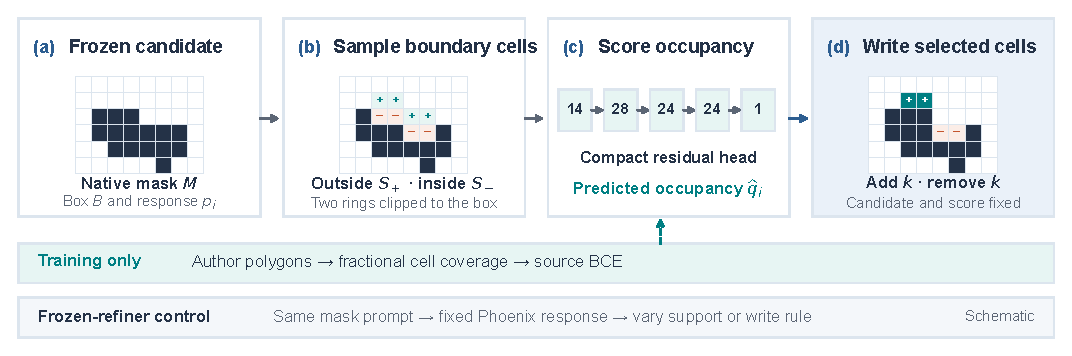
\includegraphics[width=\textwidth]{figures/cvpr_20261126/matched_budget_pipeline.pdf}
\caption{Panel (a) fixes the detector output. Panels (b) and (c) define sampled cells and estimate occupancy. Panel (d) shows the independent write at equal signed counts. The lower lane shows the frozen-refiner control. Fig.~\ref{fig:signed-allocation} illustrates the separate fixed-total allocation.}
\label{fig:native-boundary}
\end{figure*}

\section{Related Work}
\label{sec:related-work}

\subsection{SAR ship masks and native-grid boundary supervision}
HRSID and the polygon subset of SSDD made it possible to assess individual ship footprints on public SAR images \cite{hrsid,ssdd}. SRNet aligns elongated ships within rotated boxes, and DRSNet uses cross-attention to combine two scales within rotated regions \cite{rsdd,drsnet}. Later architectures use scattering key points, edge-aware alignment, geometry-aware proposals and global or channel context to improve the features from which detections and masks are predicted \cite{gao2024,aranet,dacf,gcie,dsr}. GLDet treats local gradients as a cue for ship detection \cite{gldet}. This progression improves mask generation or its upstream localization. Our experiments address the case where the candidate, score and native mask have already been produced. For this fixed input, the area of the intersection between a cell and the released polygon supplies a target for boundary scoring, including cells intersected only partly by the outline.

\subsection{Area-preserving exchanges and mask decisions}
Atkinson's subpixel mapping selects foreground and background subpixels by distance-weighted spatial attraction and swaps their labels if this increases spatial correlation, preserving the coarse class proportion \cite{atkinson}. Xu and Huang extend spatial and temporal exchanges to land-cover mapping \cite{xu}. RankSEG derives posterior ranking and foreground-volume selection for overlap-based semantic segmentation \cite{rankseg}. RankSEG-DEP uses spatially localized dependence to account for correlations between labels \cite{rankdep}. Our comparisons apply the decision criteria to edits of a retained instance. The original mask defines the two endpoint sets, and the realized candidate budget fixes the number of cells that can change. This allows us to isolate the effect of positional coupling from the effects of point scoring and changing mask area.

\subsection{Local and whole-mask refinement}
PointRend samples uncertain positions during iterative subdivision, SegFix uses interior predictions to correct boundary labels, and Boundary Patch Refinement predicts updates in image and mask patches \cite{pointrend,segfix,bpr}. RefineMask incorporates fine features at successive stages, and SharpContour iteratively moves contour vertices \cite{refinemask,sharpcontour}. QuBER uses estimated boundary false positives and false negatives as inputs to an RGB-D refinement decoder \cite{quber}. For SAR, Mansour \emph{et al.} use boxes from a SAR-trained detector to prompt a frozen SAM2 model \cite{mansour2026}. Phoenix and SegRefiner directly refine a supplied coarse mask \cite{phoenix,segrefiner}. A whole-mask result combines the refiner's response with the decision about which pixels to write. We keep that response fixed when varying writable support, the number of changed cells and the split between additions and removals. This design measures the cost of excessive writes separately from the refiner that generated them.

\section{Method}
\label{sec:method}

\subsection{Overview}
A frozen detector supplies each candidate's binary mask \(M\), box \(B\), confidence \(s\) and decoded foreground response \(p_i\) at native cell \(i\). The local editor samples inside and outside the contour, estimates each sampled cell's occupancy and writes \(k\) additions and \(k\) removals (Fig.~\ref{fig:native-boundary}). The three matched-count writers keep the detection identity, box, class, confidence and signed counts. They differ in the pairing constraint and the selected cells. A separate allocation experiment varies the split between additions and removals at a fixed total. In the pretrained-refiner diagnostic, the same image and mask prompt Phoenix XL1~\cite{phoenix}. Its fixed response is written under controlled support and budget.

\subsection{Native-grid sampling and fractional occupancy}
\label{sec:occupancy}
Let \(\Omega=\{0,\ldots,W-1\}\times\{0,\ldots,H-1\}\) be the \(W\)-by-\(H\) decoded grid. The native cell \(i=(x,y)\) covers \(C_i=[x,x+1)\times[y,y+1)\). We write \(M=\{i\in\Omega:M_i=1\}\) for the foreground set and use the same letter for its union of unit cells when measuring area. The box \(B=[x_1,x_2)\times[y_1,y_2)\) uses the same decoded coordinate frame. Eligibility uses \(x_1\le x<x_2\) and \(y_1\le y<y_2\) on the integer indices. D-FINE supplies its \(160\times160\) pre-crop sigmoid plane. For a stored plane of width \(W_m\), the center of column \(x\) maps to \((x+\tfrac12)W_m/W-\tfrac12\), with the analogous height map. For the CPU feature we use edge clamping, round the plane to FP16, interpolate bilinearly in FP32, then round the sampled value to FP16. This feature is evaluated separately from the detector's CUDA hard-mask path. RF-DETR uses the interpolated logits before applying the sigmoid. The sign of the edit comes from \(M_i\), including pixels where the sampled response and the saved native mask disagree.

For \(32\le |M|<1024\), denote one dilation and erosion by \(\delta\) and \(\varepsilon\). They use a \(3\times3\) square and a zero exterior. The two-layer pools are
\begin{equation}
\begin{aligned}
 \mathcal B_+ &= \bigl(\delta^2(M)\setminus M\bigr)\cap B\cap\Omega,\\
 \mathcal B_- &= \bigl(M\setminus\varepsilon^2(M)\bigr)\cap B\cap\Omega .
\end{aligned}
\label{eq:native-bands}
\end{equation}
In each pool, a pixel in the first dilation or erosion ring has layer \(\ell_i=1\); the additional ring has \(\ell_i=2\). We choose the first \(n=\min(32,|\mathcal B_+|,|\mathcal B_-|)\) entries on each side ordered by \((|p_i-\tfrac12|,yW+x)\). The resulting sets are \(S_+\) and \(S_-\). Masks outside the stated area range and masks with \(n=0\) pass through. Fig.~\ref{fig:occupancy-stage} traces the positions from native geometry to the occupancy estimate.

\begin{figure}[t]
\centering
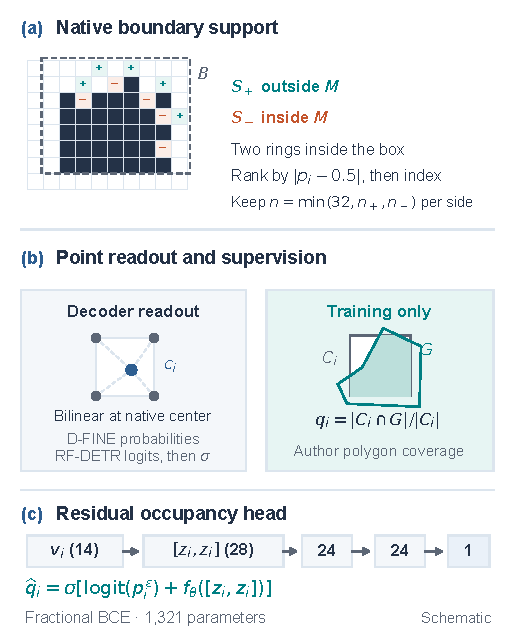
\includegraphics[width=\columnwidth]{figures/cvpr_20261126/method_native_occupancy.pdf}
\caption{Native-grid boundary support and point supervision. Outside endpoints can be added, and inside endpoints can be removed. At source training time the polygon contributes a fractional target in each unit cell. The detector response supplies the initial logit for the small learned residual.}
\label{fig:occupancy-stage}
\end{figure}

For source training, a candidate supplies targets only if it has a nonignored COCO match at raster IoU 0.50 and a valid reference polygon \(G\). The fraction of cell \(i\) inside \(G\) is
\begin{equation}
 q_i=\frac{|C_i\cap G|}{|C_i|}\in[0,1].
 \label{eq:fractional-target}
\end{equation}
The occupancy head takes the same 14 measurements at every additive and subtractive endpoint,
\begin{equation}
\begin{aligned}
 v_i=\bigl(&p_i,M_i,\ell_i,d_i,\bar x_i,\bar y_i,\nu,\eta,s,\\
           &L_i,\bar L_{3}(i),\bar L_{5}(i),\Delta_x L_i,\Delta_y L_i\bigr)^{\!\top}.
\end{aligned}
\label{eq:endpoint-features}
\end{equation}
Here \(d_i\) is the Euclidean distance to the nearest native cell of the opposite class, with a background exterior. The location features \(\bar x_i=(x-x_1)/(x_2-x_1)\) and \(\bar y_i=(y-y_1)/(y_2-y_1)\) use the candidate box. The candidate-level features are the log area \(\nu=\log_2|M|\), the occupied fraction \(\eta=|M|/|B\cap\Omega|\) and the detector confidence \(s\). In \(\eta\), the denominator counts native indices inside the clipped box.

For decoded channels \(R_i,G_i,B_i\), we use \(L_i=(0.299R_i+0.587G_i+0.114B_i)/255\). The local appearance terms are
\begin{equation}
 \bar L_w(i)=\frac{1}{w^2}\sum_{j\in\mathcal N_w(i)}L_j,\qquad
 \Delta_x L_i=\frac{L_{x+1,y}-L_{x-1,y}}{2},
 \label{eq:appearance-features}
\end{equation}
where \(\mathcal N_w(i)\) is the \(w\times w\) neighborhood centered at \(i\), with replicated edge values. The vertical difference uses the two neighboring rows with the same boundary convention. These features operate on the intensities of the distributed image rendering. The editor admits candidates from their predicted masks at inference. The AP evaluation retains all candidate slots.

For each training-source group \(j\), let \(E_j\) average the point observations from that group. The componentwise center and squared scale are
\begin{equation}
 \mu=\frac{1}{J}\sum_{j=1}^{J}E_j[v],
 \quad \sigma_v^2=\frac{1}{J}\sum_{j=1}^{J}E_j[v^2]-\mu^2.
 \label{eq:group-standardization}
\end{equation}
The implementation clips negative roundoff before taking the square root and uses unit scale wherever the resulting scale is below \(10^{-12}\). Let \(z_i=(v_i-\mu)/\sigma_v\), with the just-described scale substitution, and \(p_i^\epsilon=\operatorname{clip}(p_i,10^{-4},1-10^{-4})\). The point head is
\begin{equation}
 \widehat q_i=\operatorname{sigmoid}\!
   \left(\operatorname{logit}(p_i^\epsilon)+f_\theta([z_i,z_i])\right).
 \label{eq:occupancy-head}
\end{equation}
Here \(f_\theta\) maps \(28\to24\to24\to1\) through two ReLU hidden layers. The duplicated input keeps the parameter budget identical to the partner-context control, giving 1,321 parameters including biases. The final affine layer starts at zero, so the initial output follows the clipped decoder response.

With \(m\) sampled pairs \((a_j,d_j)\), training minimizes
\begin{equation}
\begin{split}
 \mathcal L_{\mathrm{occ}}
   &= \frac{1}{2m}\sum_{j=1}^{m}
       \left[\ell(q_{a_j},\widehat q_{a_j})+
             \ell(q_{d_j},\widehat q_{d_j})\right],\\
 \ell(q,\hat q)&=-q\log\hat q-(1-q)\log(1-\hat q).
\end{split}
\label{eq:occ-loss}
\end{equation}
An update first samples source groups uniformly, then samples a pair within each chosen group. The optimizer uses 200 AdamW updates with batch size \(m=64\) pairs, learning rate 0.002 and weight decay 0.01. Each FIT109 development fold excludes its own source prefixes from fitting and standardization. Transfer uses the all-FIT109 fit with both weights and scaling frozen.

\subsection{Endpoint Selection at Equal Signed Counts}
\label{sec:selection}
We use \(F\), \(L\), and \(I\) for distance-first pairing, bounded re-pairing, and independent endpoint selection, respectively. The unedited detector output is \(N\).
List \(S_+\) and \(S_-\) in row-major order as \(a_j\) and \(d_j\). Fixed pairing first solves
\begin{equation}
\pi^\star\in\arg\min_{\pi\in\mathfrak S_n}
  \sum_{j=1}^n\|a_j-d_{\pi(j)}\|_2^2 .
\label{eq:fixed-assignment}
\end{equation}
We keep the assignment returned by SciPy on this integer cost matrix. The fixed writer ranks the pair gains \(\widehat q_{a_j}-\widehat q_{d_{\pi^\star(j)}}\) in descending order with addition-row ties. It keeps positive gains up to \(K=\min(8,\lfloor |M|/10\rfloor,n)\). Denote the realized count by \(k\), including the case \(k=0\). At this same count the independent writer solves
\begin{equation}
\max_{\substack{A\subseteq S_+,\,D\subseteq S_-\\ |A|=|D|=k}}
  \left(\sum_{i\in A}\widehat q_i-\sum_{i\in D}\widehat q_i\right).
\label{eq:independent-estimated-gain}
\end{equation}
This selects the highest occupancies on the addition side and the lowest on the removal side, breaking ties by the original pairing-row ordinal. The natural-count comparison retains positive gains under the independent ranks up to \(K\). Figure~\ref{fig:selection-stage} illustrates the fixed-count comparison.

The bounded writer tests whether reassigning partners accounts for the gain while preserving the maximum individual displacement. For \(k>0\), let \(H_{\rm fix}\) contain the \(k\) accepted pairs of the distance-first writer. Set \(\rho^2=\max_{(a,d)\in H_{\rm fix}}\|a-d\|_2^2\). On the graph with edges satisfying \(\|a-d\|_2^2\le\rho^2\), the bounded writer solves
\begin{equation}
\max_{\substack{H\ \text{matching}\\ |H|=k}}
\sum_{(a,d)\in H}(\widehat q_a-\widehat q_d).
\label{eq:bounded-endpoint-matching}
\end{equation}
Each site appears at most once. If the independent endpoint sets admit such a matching, we use them. Otherwise we solve \eqref{eq:bounded-endpoint-matching} by unit-capacity minimum-cost flow. The cap applies to individual edges. The total squared distance and connectivity can vary. The accepted distance-first assignment is feasible for the bounded objective. Removing the cap allows any two endpoint sets of the same size. Therefore the estimated gain can only increase across these three choices.

\begin{figure*}[!t]
\centering
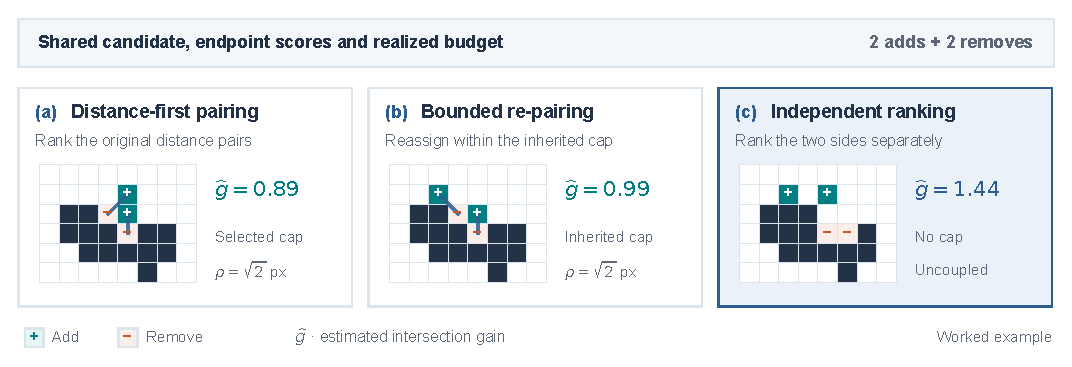
\includegraphics[width=\textwidth]{figures/cvpr_20261126/method_bounded_selection.pdf}
\caption{Three writers at the same signed counts. The bounded writer re-pairs sites under the inherited displacement cap. Independent selection removes this cap. The worked example marks the two additions and removals in each output. The value \(\widehat g\) is the estimated intersection gain.}
\label{fig:selection-stage}
\end{figure*}

On the decoded grid, let \(P=|M|\), \(T=|G|\) and \(I=|M\cap G|\) in pixel-area units, with \(U=P+T-I\). Unit cells let the signed sums of fractional coverage express the exact change in intersection. For the write \((M\setminus D)\cup A\), define
\begin{equation}
\begin{aligned}
d &= |A|-|D|,\\
g &= \sum_{i\in A}q_i-\sum_{i\in D}q_i .
\end{aligned}
\label{eq:intersect-changes}
\end{equation}
The resulting overlap is \((I+g)/(U+d-g)\). Subtracting the original IoU gives
\begin{equation}
\begin{aligned}
\Delta\mathrm{IoU}
 &= \frac{(P+T)g-Id}{U(U+d-g)},\\
\left.\Delta\mathrm{IoU}\right|_{d=0}
 &= \frac{(P+T)g}{U(U-g)}.
\end{aligned}
\label{eq:variable-area}
\end{equation}
With \(k\) additions and \(k\) removals, exactly \(2k\) labels change and the mask area remains \(P\). The derivative of the edited IoU with respect to \(g\) is \((P+T)/(U-g)^2>0\), so the true intersection gain determines the overlap ordering at this count.

The advantage in Eq.~\eqref{eq:independent-estimated-gain} is computed from estimated occupancy. Let \(g_{\rm ind}\) and \(g_{\rm pair}\) be the true gains for independent selection and distance pairing. Let \(\mathcal D\) be the symmetric difference between the two sets of edited sites. Subtracting the two gain estimates cancels edits common to both policies. Since the estimated independent gain is at least the estimated paired gain,
\begin{equation}
 g_{\rm pair}-g_{\rm ind}
 \le \sum_{i\in\mathcal D}|\widehat q_i-q_i|
 \le 4k\max_{i\in S_+\cup S_-}|\widehat q_i-q_i|
 \label{eq:selection-error}
\end{equation}
for \(k>0\). Thus prediction errors at cells on which the policies disagree can reverse the ordering of true overlap. COCO AP also permits reassignment at every raster IoU threshold while keeping the confidence order fixed.

\subsection{Dual-reference allocation at a fixed total flip count}
\label{sec:variable-sign}
The equal-count comparison holds predicted area fixed to isolate the locations of the edits. A separate experiment allows the area to change at the original total count. We fix the D-FINE candidate, its endpoint support and the count \(k_s\) from dynamic attraction. The static-attraction write \(S\) is the incumbent. Let \(E=S_+\cup S_-\), \(P=|M|\), and \(\hat q_{ir}\) be occupancy at sampled cell \(i\) for reference \(r\). The two-output head maps \(28\to24\to24\to2\) with the duplicated 14-dimensional input and a zero-initialized residual output. Its 1,346 parameters include biases. The FIT sample contains 848 common positive-budget candidates from 447 images in 439 exact decoded groups. Each of the 1,000 AdamW updates samples 64 candidates through groups and then images. The loss is the average pointwise binary cross-entropy over the two reference labels, with equal weight per sampled candidate. A single fitted head supplies both comparisons at each seed.

The surrogate reference area and native intersection are
\begin{equation}
\begin{aligned}
 \hat T_r&=|M\setminus E|+\sum_{i\in E}\hat q_{ir},\\
 \hat I_{r0}&=|M\setminus E|+\sum_{i\in E\cap M}\hat q_{ir}.
\end{aligned}
\label{eq:dual-area-proxy}
\end{equation}
The approximation uses saved native foreground outside the sampled sites. For an addition set \(A\subseteq S_+\) and removal set \(D\subseteq S_-\), let \(g_r=\sum_{i\in A}\hat q_{ir}-\sum_{i\in D}\hat q_{ir}\). The surrogate overlap is
\begin{equation}
 \hat f_r(A,D)=
 \frac{\hat I_{r0}+g_r}{P+|A|-|D|+\hat T_r-\hat I_{r0}-g_r}.
 \label{eq:dual-est-iou}
\end{equation}
For each feasible split \(a=|A|\), \(|D|=2k_s-a\), the two sides are ranked under eleven mixtures of the two occupancies, descending for additions and ascending for removals. Within each split we compare the combinations of the resulting sites, including the incumbent endpoints where their count permits. The selector maximizes the smaller of the two estimated IoU improvements over \(S\). Score ties favor the incumbent and then smaller changes in the signed allocation. The control uses the same objective and the same proposal construction within each available split. It evaluates the single split \(a=k_s\). A restricted control permits \(a=k_s-1,k_s,k_s+1\) when feasible. Every writer flips exactly \(2k_s\) cells and retains the original detection and score (Fig.~\ref{fig:signed-allocation}). We also evaluate the mean-IoU and raw-intersection objectives over the full split range. The score in Eq.~\eqref{eq:dual-est-iou} is the RankIoU-RMA ratio~\cite{rankrma} on this restricted support. To test the ratio approximation, we keep the entire signed menu and replace it with
\begin{equation}
 \hat f^{\mathrm{E}}_r(W)=\mathbb{E}[I_r(W)]\,
     \mathbb{E}\!\left[(|W|+Z_r(W))^{-1}\right],
 \label{eq:exact-iou-signed}
\end{equation}
where \(W\) is the edited mask, \(I_r(W)\) is its overlap with the random reference, and \(Z_r(W)\) sums the occupancies of sampled sites outside \(W\). Native labels beyond \(E\) are fixed. Conditional independence within each reference factors the numerator from the random union increment, as in RankIoU~\cite{rankseg}. We compute the reciprocal moment by Poisson-binomial convolution and compare the smaller expected gain across the two references. The exact and ratio criteria use identical static anchors.

\begin{figure*}[!t]
\centering
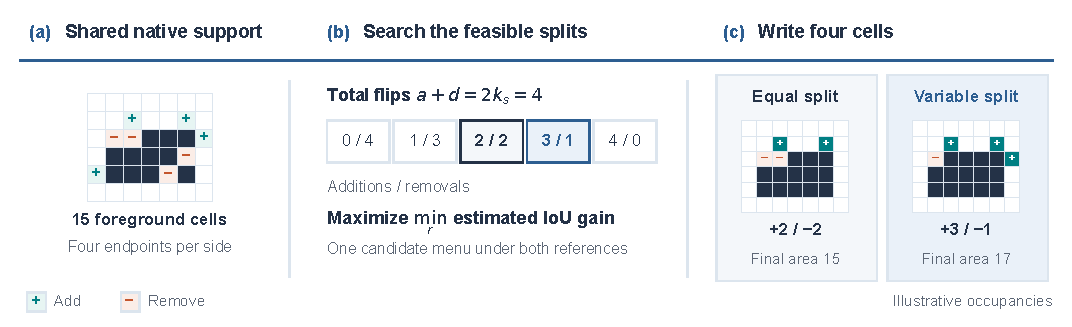
\includegraphics[width=\textwidth]{figures/cvpr_20261126/method_signed_allocation.pdf}
\caption{Allocation at a fixed total in an illustrative example. The available splits share writable endpoints. The equal split adds two cells and removes two. Maximizing the smaller predicted IoU gain across two references selects three additions and one removal in this example. Both outputs flip four cells, with different final areas.}
\label{fig:signed-allocation}
\end{figure*}

\subsection{Support and signed allocation for a frozen general refiner}
\label{sec:phoenix}
The original binary mask and decoded image prompt Phoenix XL1~\cite{phoenix}. After five refinement iterations, the selected author's mask hypothesis has native foreground probabilities \(r_i\). We change the writing policy on this one response. The allowed cells \(\mathcal W\) are either \(S_+\cup S_-\) or the complete native grid \(\Omega\). For a threshold writer, the author's binary decision replaces \(M_i\) at sites in \(\mathcal W\), including its decision when \(r_i=0.5\). All other cells are retained.

The count writer uses \(2k_{\mathrm{att}}\) flips per candidate. Here \(k_{\mathrm{att}}\) is the realized exchange count of dynamic spatial attraction~\cite{atkinson}, distinct from the learned paired count \(k\). For the current foreground \(M_\tau\) after \(\tau\) exchanges, attraction at \(i\) is
\begin{equation}
 h_\tau(i)=\sum_{j\in M_\tau} e^{-\rho_{ij}/5}
                      \mathbf{1}\{0<\rho_{ij}\le 5\},
 \quad \rho_{ij}=\lVert i-j\rVert_2 .
 \label{eq:dynamic-attraction}
\end{equation}
Each exchange selects the highest-attraction unused addition site and the lowest-attraction unused removal site, resolving ties by the original endpoint ordinal. The policy updates \(M_\tau\) and retires both sites. It stops when their attraction difference does not exceed \(10^{-12}\) or the count reaches \(K\). Static attraction uses the initial \(h_0\) at the same realized count.

For \(i\in\mathcal W\), let \(u_i^+=r_i-\tfrac12\) on original background and \(u_i^-=\tfrac12-r_i\) on original foreground. Let \(u_{(j)}^+\) and \(u_{(j)}^-\) be the respective descending orders. For \(a\) additions, the resulting score is
\begin{equation}
 F_\mathcal{W}(a)
 =\sum_{j=1}^{a}u^+_{(j)}
   +\sum_{j=1}^{\,2k_{\mathrm{att}}-a}u^-_{(j)} .
 \label{eq:writer-quota}
\end{equation}
The count writer chooses the feasible integer \(a\) maximizing \(F_\mathcal W\), with both prefix lengths constrained by the number of available cells on their side. Equal-objective splits favor the smallest absolute area change, then fewer additions. Within each side, ties follow the original endpoint ordinal and then row-major order for remaining cells. Exact counts may require writing a nonpositive margin. The balanced narrow comparison fixes \(a=k_{\mathrm{att}}\) and retains the same within-side ranks. The four factorial arms share the positive-budget candidates and probabilities. Original masks are retained at all other candidate slots.

\begin{figure}[t]
\centering
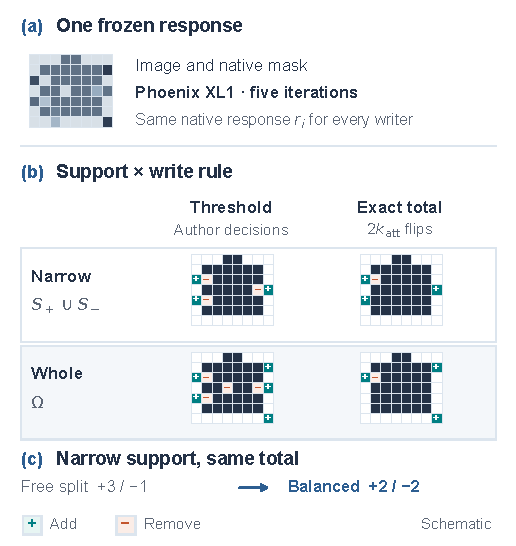
\includegraphics[width=\columnwidth]{figures/cvpr_20261126/method_phoenix_controls.pdf}
\caption{Frozen Phoenix control. Its response is shared by two choices of writable support and two writing rules. The balanced narrow comparison matches the same total count and assigns half to each side to isolate the signed split.}
\label{fig:phoenix-stage}
\end{figure}

For any evaluation statistic \(Y\), the effect of the count rule on whole support is \(Y_{\mathrm{whole,count}}-Y_{\mathrm{whole,thr}}\). Subtracting \(Y_{\mathrm{narrow,count}}-Y_{\mathrm{narrow,thr}}\) gives the support-by-rule interaction. Changing the split while holding support and total count fixed addresses a different question. Equations~\eqref{eq:intersect-changes} and \eqref{eq:variable-area} specify why the same number of changes can produce different intersection and area errors.

\section{Experimental Protocol}
\label{sec:protocol}
\subsection{Datasets and data partitions}
HRSID~\cite{hrsid}, Instance-RSDD~\cite{rsdd} and PSeg-SSDD~\cite{ssdd} provide ship instance reference polygons. SAR-SSP provides raster instance IDs~\cite{slgsea}. In the matched-position transfer experiments, the HRSID detector and HRSID fractional-occupancy head are frozen before evaluating the target images. The SAR-SSP signed-allocation comparison instead uses the frozen HRSID D-FINE detector and the dual-reference BCE head fitted on the SSDD training split. A separate PSeg experiment fits a target head while retaining the same PSeg-trained detector used with the source head. UEIKAP releases outlines for selected hulls, on which we measure coverage and overlap.

\begin{table*}[t]
\centering
\caption{Evaluation cohorts. DEV705 and the HRSID official allocation have prior development exposure. Gaofen-3 is a subset of the 740-chip test allocation. The 42-chip view is nested in the reserve. The overlap-excluded PSeg view retains 222 of the 232 official test images.}
\label{tab:cohorts}
\footnotesize
\renewcommand{\arraystretch}{1.19}
\setlength{\tabcolsep}{5pt}
\begin{tabular}{@{}p{0.26\textwidth}rrp{0.23\textwidth}p{0.30\textwidth}@{}}
\toprule
Dataset and view & Images & Hulls & Source grouping & Evaluation design \\
\midrule
HRSID DEV705 & 705 & 1,782 & 28 filename prefixes & Detector-held-out source development \\
HRSID official & 1,962 & 5,922 & -- & Historical reevaluation with overlap and empty-raster checks \\
\addlinespace[1.5pt]
Instance-RSDD author test & 740 & 872 & 112 acquisition groups & Frozen transfer. Gaofen-3 view has 583 images, 631 outlines, 76 groups \\
Instance-RSDD parent reserve & 74 & 81 & 13 additional parent scenes & Frozen transfer. Date-separated view has 42 images from eight parents \\
PSeg-SSDD official & 232 & 546 & Decoded-image groups & Frozen transfer. Exact-overlap sensitivity has 222 images \\
SAR-SSP author validation & 232 & 139 & 31 AIR-SARShip-1.0 parent scenes & Frozen transfer with raster masks. Author train and validation tiles share parents \\
\addlinespace[1.5pt]
UEIKAP reserve & 108 & 139 & 18 Sentinel-1 acquisitions & Case-focused author hull masks \\
UEIKAP additional acquisitions & 342 & 528 & 13 Sentinel-1 acquisitions & Case-focused author hull masks \\
\bottomrule
\end{tabular}
\end{table*}

The official HRSID training split contains 3,642 images. The D-FINE E24 detector was trained on 2,937 of these images. The point head was developed with five-fold source-prefix cross-fitting on FIT109 within that population, then refitted and frozen before target evaluation. DEV705 comprises 705 images from 28 filename prefixes, with zero exact encoded or RGB-content overlap and no filename-source-prefix overlap with the detector fitting population. Of these prefixes, 27 contribute to the 1,461 eligible RF-DETR 5202 matches. The prefixes serve as acquisition proxies, and DEV705 has prior development exposure.

The HRSID official PNG test split contains 1,962 images and 5,922 annotations. Four annotations rasterize to empty masks. Two test images match FIT exactly and one pair within the test split is identical. Before scoring, we fixed a primary evaluation on the full set and sensitivities excluding the four empty raster annotations or the three exact-identity images. The project previously used this split for model selection. We report the frozen reevaluation as a historical comparison on the official allocation.

For PSeg, the 187-image diagnostic view and its 182-image exact-decode sensitivity are reported separately from the 232-image historical official split. For Instance-RSDD, document counts follow the obtained source files. The sensor and parent subsets retain the source-only checkpoint and the original release annotations. The 74-chip reserve uses new parent IDs relative to the 740-chip test evaluation. The nested 42-chip reserve additionally excludes shared sensor--date keys. It retains 25 chips from three TerraSAR-X parent scenes whose rounded centers are shared with earlier test scenes. Excluding parents flagged by either metadata screen leaves 17 eligible matches in five parent groups, below the 20-match and eight-group criterion. Geographic and orbital independence remain unverified. The two Sentinel-1 reviews use the authors' case-focused hull annotations and the documented acquisition identities.

\subsection{Implementation and hardware}
We evaluate frozen D-FINE-seg-S~\cite{dfine} and RF-DETR~\cite{rfdetr} detector fits using their respective native mask paths. The 24-epoch D-FINE HRSID run made 17,640 optimizer updates. Its author inference uses a 640-pixel input, 300 queries, box NMS at 0.70 and a mask threshold of 0.50. RF-DETR uses author version 1.12.0, the 576-pixel validation transform, 164 queries and joint top-100 ranking before retaining ship-class slots. The detectors therefore contribute different candidate pools. Each paired comparison reuses candidates from the same detector and run. The HRSID fractional point heads fit on FIT109 for 200 updates under the source-group sampling in Section~\ref{sec:occupancy}. The dual-reference BCE fit follows Section~\ref{sec:variable-sign}. The two RF-DETR fits share HRSID training images and initial weights and differ in downstream seed (5202 or 5203). Point-head repeats use the declared feature and fitting budgets.

Frozen detector captures use CUDA. The RF-DETR verification runtime uses PyTorch 2.10.0 and CUDA 13.0. Polygon scoring uses pycocotools and the original coordinate geometry. Timing tests for the local writer and PointRend use an Intel Core i7-13700KF with inputs in memory and one numerical thread per pass. Frozen Phoenix XL1 inference uses four two-thread CPU workers on DGX Spark, batches of up to two masks, and the same five-iteration author setting for the writer comparisons. We report detector capture, refinement and separate scoring costs in their observed settings.

\subsection{Evaluation metrics}
\label{sec:metrics}
Let \(\mathcal T=\{0.50,0.55,\ldots,0.95\}\) be the raster mask IoU thresholds and \(\mathcal R=\{0,0.01,\ldots,1\}\) the recall levels. For \(t\in\mathcal T\), let \(\mathrm{TP}_t(j)\) and \(\mathrm{FP}_t(j)\) count the cumulative matches and unmatched predictions among the first \(j\) nonignored ranked results. Within each image the evaluator retains at most 100 predictions, uses the original scores and assigns matches to reference masks at threshold \(t\). The cumulative counts then use detections pooled across images in score order. Write \(N_G\) for the number of eligible references, and
\begin{equation}
 P_t(j)=\frac{\mathrm{TP}_t(j)}{\mathrm{TP}_t(j)+\mathrm{FP}_t(j)},
 \qquad R_t(j)=\frac{\mathrm{TP}_t(j)}{N_G}.
\end{equation}
For the single ship class, the \href{https://github.com/cocodataset/cocoapi/blob/master/PythonAPI/pycocotools/cocoeval.py}{COCO evaluator} uses the precision envelope \(P_t^*(r)=\max_{j:R_t(j)\ge r} P_t(j)\), with zero if the recall level is unreached. The scores are
\begin{equation}
\begin{aligned}
 \mathrm{AP}_t&=\frac{1}{|\mathcal R|}\sum_{r\in\mathcal R}P_t^*(r),\\
 \mathrm{AP}&=\frac{1}{|\mathcal T|}\sum_{t\in\mathcal T}\mathrm{AP}_t,\qquad
 \mathrm{AR}_{100}=\frac{1}{|\mathcal T|}\sum_{t\in\mathcal T}\max_j R_t(j).
\end{aligned}
\label{eq:coco-metrics}
\end{equation}
AP75 and AP90 are the \(t=0.75\) and \(t=0.90\) slices. Small-mask AP uses the COCO small area bin through \(32^2\) native pixel-area units.

For hull geometry we establish the original nonignored raster-IoU-0.50 match once and freeze its candidate. Let \(M'\) be its edited mask in the native grid, \(P'=|M'|\), \(I'=|M'\cap G|\) and \(T=|G|\). We intersect the union of native unit cells with the continuous annotated polygon \(G\) and report
\begin{equation}
 \mathrm{IoU}_{\mathrm{cont}}=\frac{I'}{P'+T-I'},\quad
 F_{\mathrm{P}}=\frac{P'-I'}{T},\quad F_{\mathrm{N}}=\frac{T-I'}{T}.
 \label{eq:fixed-geometry-metrics}
\end{equation}
The last two quantities normalize the false-positive and missed area by the reference area. To estimate a paired effect, we average per-hull differences \(\Delta_{ji}\) within the \(G_b\) contributing source groups and take
\begin{equation}
 \overline\Delta=\frac{1}{G_b}\sum_{j=1}^{G_b}
                 \frac{1}{n_j}\sum_{i=1}^{n_j}\Delta_{ji},
 \label{eq:paired-acquisition-effect}
\end{equation}
where \(n_j\) is the analyzed hull count in group \(j\). Geometry intervals use paired group resampling, typically 4,096 draws. Instance-RSDD reserve views keep parent weights and resample sensor--date blocks. PSeg groups are decoded-image equivalence groups. In the 183-image dual-reference comparison, we first average raster IoU over all annotated hulls in each image with native misses set to zero. Images then receive equal weight within each decoded group. The denominators are 411 and 410 hulls for PSeg and SPSD, respectively. When several heads share the same native matches, their effects are averaged within each group first. For SAR-SSP, Eq.~\eqref{eq:paired-acquisition-effect} uses mother-scene groups and \(\mathrm{IoU}_{\mathrm{raster}}=|M'\cap G_{\mathrm{r}}|/|M'\cup G_{\mathrm{r}}|\), where \(G_{\mathrm{r}}\) is the released set of foreground cells for an instance. In the SAR-SSP and case-focused UEIKAP all-hull estimates, unmatched references contribute zero change. UEIKAP also reports independently rematched coverage. COCO AP uses the benchmark views released for instance evaluation. Seed ranges summarize the observed fits.

For the frozen Instance-RSDD masks, we also measure Boundary IoU~\cite{boundaryiou} on the original matches. Let \(B_d(X)\) contain the foreground cells removed by \(d\) successive \(3\times3\) erosions of binary mask \(X\), with zero outside the chip. We compute \(|B_d(M')\cap B_d(G_{\mathrm r})|/|B_d(M')\cup B_d(G_{\mathrm r})|\) for \(d=1\) and \(d=2\) native pixels. Differences are averaged within each matched hull across the corresponding heads, then within parent scenes and equally over those scenes. We use 4,096 paired parent resamples and additionally resample sensor--date blocks in the reserve. The thickness is fixed in pixels and the geometry uses a fixed native assignment.

The fixed-match HRSID RF-DETR counts at the strict threshold use continuous IoU \(>0.90\). D-FINE and the stated PSeg RF-DETR counts include equality. These counts and COCO AP90 serve different functions. One sensitivity comparison changes the overlap matrix from raster mask IoU to polygon--cell IoU while keeping candidate order, annotation support, area bins and the evaluation rules fixed.

\section{Quantitative Results}
\label{sec:quantitative}

\begin{table*}[t]
\centering
\caption{Independent endpoint selection relative to fixed distance pairing at identical candidate, score and signed budget. AP changes are point estimates. Continuous-IoU intervals use paired source-group resampling. The Gaofen-3 fits share evaluation scenes.}
\label{tab:primary-quant}
\footnotesize
\renewcommand{\arraystretch}{1.17}
\setlength{\tabcolsep}{7pt}
\begin{tabular}{@{}llrrrl@{}}
\toprule
\multicolumn{2}{@{}l}{Evaluation scope} &
\multicolumn{2}{c}{Sample size} &
\multicolumn{2}{c@{}}{Change (points)} \\
\cmidrule(lr){1-2}\cmidrule(lr){3-4}\cmidrule(l){5-6}
Cohort & Detector & Images & Eligible fixed matches & Mask AP & Continuous IoU [95\% CI] \\
\midrule
HRSID DEV705 & D-FINE E24 & 705 & 1,447 & \(+0.811\) & \(+0.529\ [0.455,0.597]\)\\
 & RF-DETR 5202 & 705 & 1,461 & \(+0.906\) & \(+0.639\ [0.548,0.743]\)\\
 & RF-DETR 5203 & 705 & 1,465 & \(+0.838\) & \(+0.583\ [0.488,0.678]\)\\
HRSID official & RF-DETR 5202 & 1,962 & -- & \(+1.216\) & --\\
\addlinespace[2pt]
Instance-RSDD Gaofen-3 & RF-DETR 5202 & 583 & 425 & \(+0.483\) & \(+0.259\ [0.194,0.322]\)\\
 & RF-DETR 5203 & 583 & 425 & \(+0.299\) & \(+0.196\ [0.136,0.253]\)\\
Instance-RSDD reserve & RF-DETR 5202 & 74 & 47 & \(+0.436\) & \(+0.318\ [0.217,0.436]\)\\
 & RF-DETR 5203 & 74 & 48 & \(+0.306\) & \(+0.267\ [0.161,0.374]\)\\
PSeg-SSDD official & D-FINE E24 & 232 & 293 & \(+0.081\) & \(+0.106\ [0.055,0.157]\)\\
\bottomrule
\end{tabular}
\end{table*}

Among the polygon cohorts in Table~\ref{tab:primary-quant}, independent selection has its largest effects on HRSID and yields smaller gains in the Gaofen-3 transfer. The within-row contrasts change only the edited locations. On the Gaofen-3 images, continuous IoU increases by 0.259 and 0.196 points for the two detector fits. PSeg-SSDD shows a smaller AP gain of 0.081 points. Table~\ref{tab:sar-ssp} reports the raster-mask cohort separately. Comparisons with spatial attraction and complete-mask refiners test performance against alternatives to distance pairing.

\subsection{Source benchmark and repeated detector fits}
\begin{table*}[t]
\centering
\caption{D-FINE E24 on HRSID DEV705. COCO AP and recall use all 70,500 original candidates. Continuous IoU gives equal weight to source groups over 1,447 eligible valid matches of 1,652 original fixed matches. All rows retain candidate ranks, scores and foreground areas. Scores are scaled by 100.}
\label{tab:dev}
\begin{tabular}{lrrrrrr}
\toprule
Mask policy & AP & AP75 & AP90 & Small AP & AR100 & Continuous IoU\\
\midrule
Raw D-FINE E24 & 48.160 & 51.507 & 0.145 & 47.196 & 54.018 & 75.798\\
Same head, fixed pairing & 48.916 & 53.453 & 0.146 & 48.017 & 54.792 & 76.258\\
Independent selection, fixed-pair count & 49.726 & 55.285 & 0.200 & 48.923 & 55.617 & 76.787\\
\midrule
Independent selection, natural count & 50.715 & 57.760 & 0.223 & 50.034 & 56.695 & 77.217\\
Native decoder ranking, natural count of independent policy & 47.951 & 50.616 & 0.126 & 46.927 & 53.765 & 75.652\\
\bottomrule
\end{tabular}
\end{table*}

The natural policy increases mask AP by 2.555 points and small-object AP by 2.838 points over raw D-FINE (Table~\ref{tab:dev}). Group-equal continuous IoU increases by 1.419 points, with paired 95\% interval \([1.265,1.587]\). All three original valid strict matches are retained, and 12 additional matches reach 0.90. COCO AP90 remains low in absolute terms.

At 83,059 swaps on 20,741 candidates, independent selection gains 0.811 AP and 0.529 continuous IoU over fixed pairing (IoU interval \([0.455,0.597]\)). The analogous five-fold FIT109 gains were 1.576 AP and 0.615 IoU. Natural selection makes 194,052 swaps, changing both coverage and count. Native decoder ranking at this count can force swaps with nonpositive predicted gains.

The second RF-DETR fit (5203) reuses the starting weights and data. Matched-count gains are positive for all three point heads (Table~\ref{tab:primary-quant}). Its natural count raises AP from 55.914 to 56.726.

\subsection{Frozen evaluation on the HRSID official split}
The official-split reevaluation uses the first E24 RF-DETR fit (5202), three frozen FIT109 point-head seeds, and 187,796 native mapped candidates. An independent replay verifies candidate identities, scores, realized edit counts and written masks. The natural policy gains 1.021 mask AP points over the native masks (Table~\ref{tab:official}), with seed effects of 1.078, 1.062 and 0.923 points. At the fixed-pair count, independent selection gains 1.216 AP, 1.958 AP75 and 1.379 small-object AP points. Its AP gains are 1.052, 1.297 and 1.299. Both comparisons remain positive for every seed when excluding empty annotations or exact image overlap. Their mean AP gains range from 1.018 to 1.029 and 1.207 to 1.216 points, respectively.

\begin{table}[t]
\centering
\caption{HRSID official allocation on frozen RF-DETR. Refined rows average three seeds. Independent fixed uses the paired count. The large head writes unequal signed counts at the independent natural total. Scores are points.}
\label{tab:official}
\footnotesize
\setlength{\tabcolsep}{3.5pt}
\begin{tabular}{@{}lrrrrr@{}}
\toprule
Policy & AP & AP75 & AP90 & AP$_{S}$ & AR100\\
\midrule
Native & 54.433 & 62.190 & 4.417 & 52.823 & 61.694\\
Paired & 54.227 & 61.862 & 4.307 & 52.570 & 61.179\\
Independent, fixed & 55.444 & 63.821 & 4.908 & 53.949 & 62.790\\
Independent, natural & 55.454 & 63.709 & 4.925 & 53.960 & 62.774\\
Large, free signs & 55.130 & 63.260 & 4.827 & 53.591 & 62.265\\
\bottomrule
\end{tabular}
\end{table}

Relative to LW=S, SU gains 0.324 AP points on average, with seed effects of \(+0.184\), \(+0.963\), and \(-0.174\). This contrast changes both the predictor and area policy. Switching from SU=F to the natural count changes mean AP by \(+0.011\) and AP75 by \(-0.112\) points. The official comparison supports a recurring cost of distance-based pairing on carrier 5202 (Table~\ref{tab:official}). On this split the independent replay establishes COCO AP. Source and transfer analyses supply the fixed-match continuous effects.

\begin{figure*}[!t]
\centering
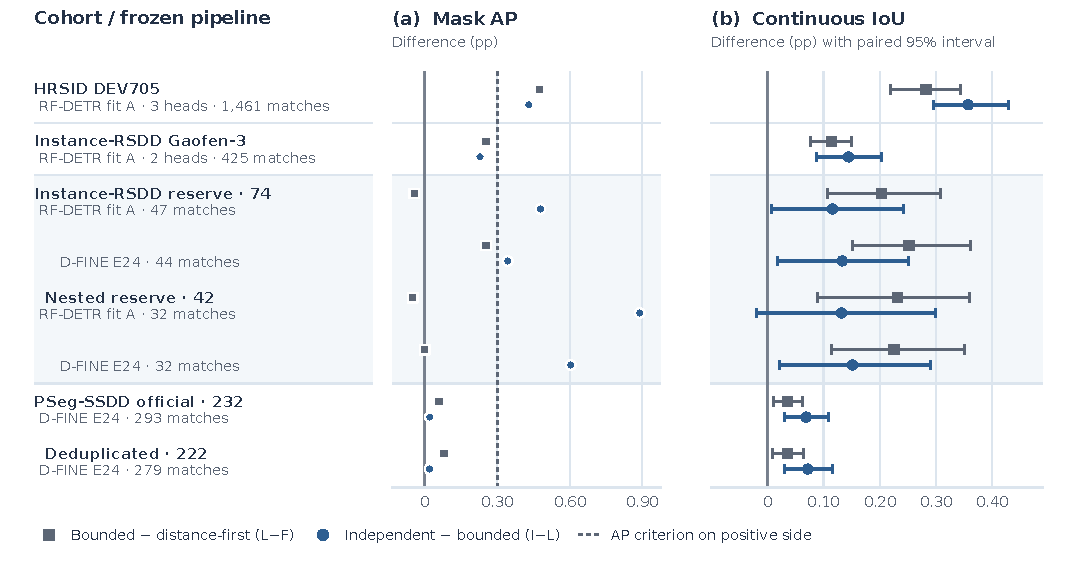
\includegraphics[width=\textwidth]{figures/cvpr_20261126/transfer_effects.pdf}
\caption{Matched-count effects of changing the pairing constraint. Squares compare bounded re-pairing with distance-first assignment (\(L-F\)); circles compare independent ranking with bounded re-pairing (\(I-L\)). Panel (a) gives mask AP point estimates, with the dashed line marking the positive-side AP advance criterion. Panel (b) gives fixed-match continuous IoU effects with paired 95\% group intervals. Each row shares the detector, head, sampled endpoints and realized signed counts across all writers. The reserve pipelines share target images and the 42-chip view is nested. Deduplication removes exact historical fitting overlaps from the PSeg-SSDD view. Counts are eligible fixed matches.}
\label{fig:transfer-effects}
\end{figure*}

\subsection{Frozen transfer to Instance-RSDD}
Instance-RSDD~\cite{rsdd} supplies hull outlines for RSDD-SAR imagery~\cite{rsddsar}. The author files contain 2,810 training and 740 test chips, compared with 2,840 and 715 in the paper. The 740 test chips contain 872 outlined vessels, and all 112 test parent scenes recur in the author training allocation. The RF-DETR fits and their occupancy heads in this comparison were fitted on HRSID only. The prespecified Gaofen-3 view represents a sensor absent from HRSID fitting (583 chips, 631 outlines and 76 acquisitions). The remaining 157 test chips are TerraSAR-X.

On Gaofen-3, the first detector's two natural policies gain 0.587 and 0.517 AP over native. AP75 rises by 1.438 and 1.230, while AP90 falls by 0.094 and 0.107. With count fixed, the corresponding AP gains over pairing are 0.482 and 0.483. Mean continuous IoU gains 0.259 points (\([0.194,0.322]\), 425 eligible matches, 68 contributing acquisitions). This is a paired mean over the two heads. The second detector, sharing initialization and point-head provenance, gains 0.240, 0.280, and 0.378 AP points at equal count. Its mean AP and IoU gains are 0.299 and 0.196 (\([0.136,0.253]\)) on its own 425 eligible matches, with 67 contributing acquisitions. Across all 740 images, natural selection gains mean AP of 0.539 and 0.435 for the two fits. The gain from freeing pairs at fixed count repeats more consistently than a large improvement over the native proposal.

The separate reserve contains 74 chips from 13 additional parents in the author training allocation. With detector 5202 and head 5217, equal-count independence gains 0.436 AP and 0.318 IoU (\([0.217,0.436]\), 47 eligible matches). The nested date-separated view contains 42 chips and 32 eligible matches. It gains 0.840 AP and 0.364 IoU (\([0.250,0.478]\)). Detector 5203 has 48 and 31 eligible matches in the two views. Its three-head means gain 0.306 and 0.529 AP and 0.267 and 0.326 IoU (\([0.161,0.374]\), \([0.166,0.460]\)). Both fits meet the 20-match and eight-parent criteria in each view. Intervals resample sensor--dates with equal parent weights. The date split probes temporal proximity within the reserve. Geographic independence is unverified.

With the original matches and signed counts frozen, the one-pixel boundary gain is positive with an interval above zero for GF-3 detector 5202 and for the 74-chip reserve (Table~\ref{tab:native-boundary}). On the same GF-3 images, the one-pixel interval for detector 5203 spans zero. Both GF-3 fits and the reserve give positive two-pixel intervals. Each eligible author and native mask has a nonempty eroded interior at both widths. The two GF-3 fits use 425 eligible matches each, in 68 and 67 parents. The reserve uses 47 matches in 12 parents. Its one-pixel independent-versus-paired interval with sensor--date blocks is \([0.231,1.243]\). Each comparison uses the original COCO predictions, scores and match identities.

\begin{table}[t]
\centering
\caption{Fixed-match boundary IoU differences in points. The first three rows compare independent ranking with distance pairing. The last compares occupancy ranking with matched-support PointRend at its own fixed signed count. Brackets give paired 95\% parent intervals.}
\label{tab:native-boundary}
\footnotesize
\setlength{\tabcolsep}{2.5pt}
\begin{tabular}{@{}lcc@{}}
\toprule
Cohort and comparison & One pixel & Two pixels\\
\midrule
GF-3, 5202 & \(+0.466\ [0.223,0.702]\) & \(+0.467\ [0.278,0.653]\)\\
GF-3, 5203 & \(+0.177\ [-0.025,0.376]\) & \(+0.255\ [0.107,0.404]\)\\
Reserve, paired & \(+0.701\ [0.180,1.233]\) & \(+0.617\ [0.236,1.001]\)\\
Reserve, PointRend & \(+0.829\ [-0.056,1.750]\) & \(+0.801\ [0.285,1.370]\)\\
\bottomrule
\end{tabular}
\end{table}

\subsection{Frozen transfer to PSeg-SSDD}
Five frozen HRSID policies share all 18,700 native candidates, including empty masks (Table~\ref{tab:ssdd}).


On DEV187, natural selection gains 0.336 AP over native and 0.278 over fixed pairing, below the 0.50 and 0.30 margins. At equal counts, independent selection gains 0.071 AP and 0.112 IoU (\([0.048,0.178]\), 209 fixed matches, 111 image groups). No match exceeds 0.90. Deduplication preserves the directions. Acquisition independence remains unverified.

On the historical official split, AP rises from 17.974 to 18.319 and AP75 from 13.015 to 14.705. At equal counts, AP exceeds fixed pairing by 0.081. Ten test images share decoded content with the historical PSeg training allocation. Excluding them yields 0.389 AP over native and 0.100 over fixed pairing. The detector and head in this transfer comparison were fitted on HRSID.

Across 293 editable matches, independent selection gains 0.106 IoU over fixed pairs (image-paired 95\% interval \mbox{\([0.055,0.157]\)}). Natural selection gains 0.228 over native (\([0.104,0.364]\)). All stay below 0.90. Oracle ranks at the learned count add 1.097 IoU points. Allowing unequal counts at the same total flips adds 2.020 more.

At the dynamic attraction count~\cite{atkinson} (73,770 exchanges, 11,054 predictions), learned ranking scores 18.331 versus 18.357 AP, gains 0.279 AP75 and loses 0.270 IoU (\([-0.440,-0.098]\)). Deduplication preserves these directions. Releasing the distance assignment helps the occupancy writer at its paired count. At the dynamic count, the same occupancy scores produce lower continuous overlap than attraction.

At the dynamic edit count on historical DEV187, the transferred HRSID head scores 69.958 AP, and dynamic attraction scores 69.113 with the same PSeg-trained RF-DETR E24. The 0.193 IoU gain misses the criterion (119-group paired 95\% interval \([-0.036,0.430]\)). Native masks score 70.694 AP, leading by 0.735 AP and 0.404 IoU (\([0.245,0.564]\)). Equal-count independent selection gains 0.279 AP and 0.097 IoU over fixed pairing (\([-0.035,0.232]\)).

On 281 matches, polygon-optimal ranks at the attraction count exceed native by 2.246 IoU and learned ranks by 2.651. Fewer flips on frozen support add 0.032 beyond this optimum, and varying area at fixed total flips adds 1.018. These reference-dependent ceilings identify recoverable overlap inside the evaluated support, with scope to improve both the rankings and the area constraint.

Refitting on 109 PSeg training images (zero decoded DEV187 overlap, 200 updates) yields 69.809 AP at the attraction count, 0.695 above dynamic, 0.150 below transfer and 0.885 below native. IoU falls 0.470 from native (\([-0.621,-0.325]\)). Deduplicated AP agrees in direction. The refit misses the replication criterion.

\begin{table}[t]
\centering
\caption{Frozen HRSID-to-PSeg-SSDD mask AP on DEV187. Float and integer use 187 images. Dedup.\ scores float polygons on 182 unique decoded images.}
\label{tab:ssdd}
\footnotesize
\begin{tabular}{@{}lrrr@{}}
\toprule
Mask policy & Float & Integer & Float, dedup. \\
\midrule
Raw D-FINE E24 & 17.897 & 16.804 & 18.261 \\
Same head, fixed pairing & 17.956 & 16.877 & 18.329 \\
Independent, fixed-policy count & 18.028 & 17.173 & 18.393 \\
\midrule
Independent, natural count & 18.234 & 17.557 & 18.620 \\
Native ranks, natural-policy count & 17.942 & 16.757 & 18.308 \\
\bottomrule
\end{tabular}
\end{table}

\subsubsection{Sensitivity to the reference masks}
SPSD~\cite{slgsea} releases ship masks for the same 232 test JPEGs. All image files are byte-identical to PSeg-SSDD. We hold the 23,200 D-FINE candidate slots, masks, ranks and edit locations fixed and score both releases. The original evaluation uses rasterized PSeg polygons. For SPSD, we derive native area and bounds from the author's raster instance IDs. Within-chip one-to-one assignment gives 544 reference pairs with median raster IoU 0.747 and median SPSD-to-PSeg area ratio 0.822. The original masks match 402 of 546 PSeg hulls and 403 of 547 SPSD hulls at mask IoU 0.50.

The equal-count independent-minus-paired AP difference changes from \(+0.081\) points on PSeg to \(-0.007\) on SPSD. Independent selection at its natural count gains \(0.344\) AP points over native on PSeg and loses \(0.491\) on SPSD. Its all-hull raster IoU effect changes from \(+0.119\) to \(-0.240\) points. The difference between IoU effects is \(-0.359\) points (\([-0.479,-0.247]\)), with the same decoded-image bootstrap draws and separate native matches for each reference. Learned ranking relative to static attraction at the same count loses \(0.086\) AP points on PSeg and \(0.946\) on SPSD. Changing the released reference thus changes the measured consequences of the same edits, without changing image content or predictions.

Of the 493 reference pairs with mutual IoU at least 0.50, 358 share a native candidate. Natural-count editing changes 262 such candidates in 137 images. For reference \(R\) its IoU effect is \(a_Rg_R\), where \(g_R\) is the signed intersection gain in Eq.~\eqref{eq:intersect-changes} and \(a_R\) is the corresponding IoU scale. The term \(\bar a(g_{\rm SPSD}-g_{\rm PSeg})\) depends only on edits to cells with conflicting reference labels. At the original 232-image weights, this term accounts for \(-0.286\) points (\([-0.388,-0.193]\)) of the \(-0.359\)-point total shift. IoU scaling on the same candidates contributes \(-0.013\) points. Assignment, reference count and unpaired hulls account for the rest. Fig.~\ref{fig:reference-disagreement} places this decomposition beside the matched-budget comparisons. The conflicting-label term is \(-0.313\) points (\([-0.440,-0.193]\)) for occupancy ranking against static attraction and \(-0.037\) points (\([-0.081,+0.006]\)) for independent selection against distance pairing. In the natural-count comparison, restricting the shared matches to reference pairs with mutual IoU of at least 0.75 leaves a \(-0.102\)-point conflicting-label term (\([-0.163,-0.046]\)) on the original image weights. The comparison measures sensitivity to two released labels and does not establish the physical outline of any individual hull.

\begin{figure*}[!t]
\centering
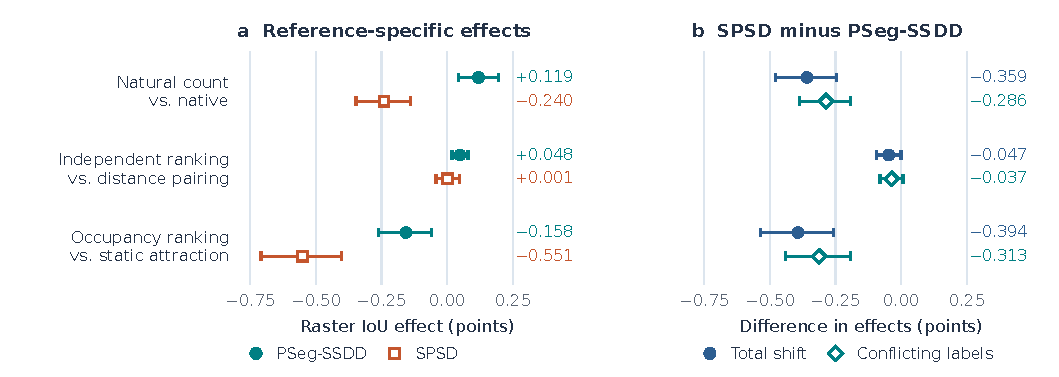
\includegraphics[width=0.98\textwidth]{figures/cvpr_20261126/reference_disagreement_effects.pdf}
\caption{Effect of exchanging the released reference masks on the same 232 SSDD images. (a) Each row compares the same two predicted masks under PSeg-SSDD and SPSD. (b) The total shift subtracts the PSeg-SSDD effect from the SPSD effect. The conflicting-label term is the contribution from edited cells on targets assigned to the same native candidate under both references. The remaining terms include IoU normalization, candidate assignment and reference composition. Intervals are paired 95\% percentile intervals from 4,096 decoded-image resamples.}
\label{fig:reference-disagreement}
\end{figure*}




\subsubsection{Variable signed allocation at the same total count}
\label{sec:variable-sign-results}
We draw the fitting candidates from 732 images in the SSDD author training allocation. The common positive-budget set spans 447 of those images. Evaluation uses 183 previously used SSDD development images in decoded-image groups excluded from fitting. Each writer flips 115,384 cells over the same 18,300 candidates. The fixed-allocation control adds and removes 57,692 cells each. The variable-IoU writer at seed 5297 makes 67,777 additions and 47,607 removals. It gains 2.461 mask AP points and 0.993 fixed IoU points (\([0.747,1.244]\)) on PSeg-SSDD. On SPSD it gains 1.782 AP and 0.580 IoU points (\([0.298,0.877]\)). The archived fixed-area BCE robust and mean writers also give smaller scores on both references. At the same full split range, the mean-IoU objective exceeds the maximin objective on PSeg-SSDD by 0.498 AP and 0.312 fixed-match raster IoU points. The corresponding SPSD differences are \(-0.044\) and \(-0.073\) points. The objective comparison therefore shows a trade-off between the two reference releases.

Let \(P_0,P_1\) and \(I_0,I_1\) denote the areas and intersections of the fixed and variable outputs against the same reference. Write \(U_j=P_j+T-I_j\), \(\bar P=(P_0+P_1)/2\), and \(\bar I=(I_0+I_1)/2\). The exact difference is
\begin{equation}
 \Delta\mathrm{IoU} =
 \frac{(\bar P+T)(I_1-I_0)-\bar I(P_1-P_0)}{U_0 U_1}.
 \label{eq:area-overlap-parts}
\end{equation}
The added intersection contributes 2.243 and 2.041 IoU points on the two references. The area terms are \(-1.250\) and \(-1.461\) points (Fig.~\ref{fig:dual-budget-effect}). The group-mean absolute area errors fall by 4.705 and 1.520 cells. Among 206 common positive-budget hulls, 182 gain intersection under both references and five lose intersection under at least one. This shows that the expanded masks recover annotated hull area on these images. The reference-area estimate in Eq.~\eqref{eq:dual-area-proxy} depends on the native foreground outside the sampled sites. Both references place about 78\% of the static-mask error outside those sites.



Table~\ref{tab:dual-sign-seeds} reports the two prespecified repeats together with the archived first fit. Each seed uses its own paired fixed and variable writers. Averaging the three seeds on the same images gives 2.299 and 1.751 mask AP points and 0.971 and 0.573 fixed IoU points on PSeg-SSDD and SPSD. The respective IoU intervals are \([0.740,1.207]\) and \([0.319,0.840]\). Each paired group draw resamples the complete vector of seed-specific differences. These intervals describe image-group variability after averaging the tested fits. All three fits share the source data and fixed detector.

On the original 5297 fit, we also substitute Eq.~\eqref{eq:exact-iou-signed} for the ratio in both signed-allocation arms. At the same total edit count, the exact variable and fixed choices differ from their ratio counterparts on 136 and 11 of 8,785 positive-budget candidates, respectively. The variable choices agree on all 206 common positive-budget matches. Mask AP and fixed-match IoU agree for each pair under both references, retaining the variable versus fixed gains. This comparison isolates the reciprocal-moment approximation under independent endpoint Bernoulli labels and deterministic native labels beyond the writable support. The spatial dependence considered by RankSEG-DEP~\cite{rankdep} would require a different joint model. For fixed signed counts, the expected intersection objective in Eq.~\eqref{eq:independent-estimated-gain} depends only on occupancy marginals by linearity.

We also fit a joint model on disjoint four-neighbor endpoint pairs. It retains the same occupancy marginals and compares local dependence with zero dependence and sign-preserving rewiring. On held FIT groups, local dependence lowers the four-state Brier loss by 0.058 and 0.089 under the two references compared with independence on the same local pairs. We freeze the coefficients and recompute exact expected IoU over the same signed menus. Of 206 common positive-budget native matches on source development, only one changes its mask relative to independence. Mask AP is identical under both references. The fixed-match raster IoU differences are zero and \(+0.00175\) points, with the latter interval including zero. Improved pair prediction had little effect on the final masks in this setting.

\begin{table}[t]
\centering
\caption{Variable allocation minus fixed allocation at identical total flips. Both policies use the same head at each seed. Values are percentage points.}
\label{tab:dual-sign-seeds}
\footnotesize
\begin{tabular}{@{}lrrrr@{}}
\toprule
 & \multicolumn{2}{c}{PSeg-SSDD} & \multicolumn{2}{c}{SPSD}\\
\cmidrule(lr){2-3}\cmidrule(lr){4-5}
Seed & AP & IoU & AP & IoU\\
\midrule
5297 & 2.461 & 0.993 & 1.782 & 0.580\\
5298 & 2.465 & 1.037 & 1.615 & 0.584\\
5299 & 1.971 & 0.882 & 1.856 & 0.555\\
\midrule
Mean & 2.299 & 0.971 & 1.751 & 0.573\\
\bottomrule
\end{tabular}
\end{table}

With the source head and policy frozen, the same fixed-total-flip comparison on 232 SAR-SSP validation chips yields \(-0.139\) mask AP and \(-0.212\) fixed IoU points (\([-0.547,0.104]\)). It changes 48 original matches from 20 parent scenes. The variable policy decreases missed area by 0.653 points of reference area (\([-1.079,-0.328]\)) and increases excess foreground area by 1.378 points (\([0.750,2.067]\)). This target uses the released native raster masks and had prior evaluation exposure. The frozen procedure does not pass its paired transfer criterion on these data. The exact expected-IoU comparison preserves the same transfer result. Although 142 of 10,393 candidates change their selected variable writes, the exact and ratio objectives give identical mask AP and fixed IoU in each allocation arm.

To locate the loss, we replayed the original candidate menu for the 50 native matches with positive edit counts and kept the same 139-hull denominator. Using the author masks to select the best action at the model's chosen split recovered 0.180 mother-scene-weighted IoU points. Searching all splits after this within-split replacement recovered a further 1.147 points. In a separate substitution, retaining the predicted winner at every split and choosing only the split using the author masks recovered 0.958 points. Replacing the reference area and static intersection by their exact values, while retaining predicted intersection changes, changed realized IoU by 0.005 points (\([-0.096,0.115]\)). The observed deficit thus leaves room to improve how the number of additions and removals is chosen. These substitutions use the author masks and describe the available actions on this cohort.

Of the 393 false foreground cells present only under variable allocation, 392 belong to the largest component containing a retained fixed-mask cell. This count agrees under four- and eight-neighbor connectivity. Net excess foreground consists of 162 cells outside the native mask and 175 native cells retained by the variable writer. The corresponding scene-weighted, reference-normalized changes are 0.667 and 0.711 points. Isolated added components account for one gained false foreground cell on the original matches.

We also replay the occupancy predictions at the exact sites where the two writes differ. On SAR-SSP, the two source-fitted outputs overestimate the intersection gain by 0.896 and 0.628 points of author reference area. The same computation against their corresponding SSDD references gives 0.089 and 0.231 points. The target area-coefficient terms are negative for both outputs and offset part of the error. This comparison is conditional on the selected edits. The two predictions share one target author mask, and the source and target estimates use their own group definitions.

\begin{figure*}[!t]
\centering
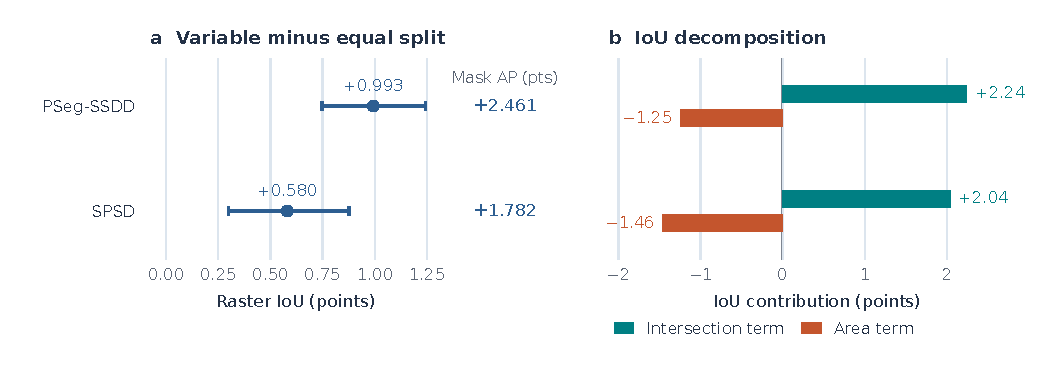
\includegraphics[width=0.98\textwidth]{figures/cvpr_20261126/dual_reference_budget_effect.pdf}
\caption{Variable versus equal addition and removal counts at an identical total number of flips. Both use the same learned occupancy, candidate stream and predicted-IoU objective. (a) Seed 5297 differences on the 183 development images. IoU intervals use 4,096 paired decoded-image-group resamples. (b) Intersection and area terms from Eq.~\eqref{eq:area-overlap-parts}. Values retain each release's native assignments and complete hull denominator.}
\label{fig:dual-budget-effect}
\end{figure*}

\subsection{Comparisons with strong ranking and full-mask alternatives}
After fixing the edit budget, the next question is whether learned scores select better cells than a geometric rule. On the 74-chip reserve, at the dynamic attraction count, occupancy gains 0.468 AP and 0.431 IoU over dynamic (\([0.213,0.662]\)), and 0.203 AP and 0.301 IoU over static (\([0.088,0.534]\)). Static still leads by 0.173 AP75. Both contrasts change 47 eligible masks in 11 sensor--date blocks. The date-separated AP gains are 0.978 and 0.478, while neither sensor stratum alone meets the exposure criterion.





Strict matches are also sensitive to how the same source polygon is represented. In the second fit on Gaofen-3, learned minus dynamic AP90 changes from \(-0.149\) under standard raster overlap to \(+0.004\) under polygon--cell overlap. The paired 95\% interval for the change is \([-0.195,0.579]\). The first fit shrinks from \(+0.279\) to \(+0.053\). The 631 outlines and the prediction identities and order are held fixed. In both fits, the mean AP advantage averaged across the ten thresholds remains positive. The strict-threshold result motivates reporting the overlap convention and match coverage alongside AP90.

At matched endpoints and counts on 74 chips, five-pass Phoenix XL1~\cite{phoenix} without its 1\% gate gains 0.308 AP (58.976) and 0.135 IoU (\([-0.026,0.277]\)) over occupancy. Substituting occupancy for only the Phoenix additions changes mean AP by \(-0.012\), while substituting only deletions changes it by \(-0.225\). Both adjusted intersection intervals cross zero. Under image-only \(\pm1\)-column shifts, the mean signed centroid response is 0.117 pixels for Phoenix and 0.070 for occupancy (paired difference 0.047, \([0.028,0.064]\), 47 hulls). The latter result measures sensitivity to image alignment on fixed proposals. Its contribution to the ranking gap on correctly aligned images remains uncertain.

Binary PointRend used HRSID FIT109 RF-DETR features, 200 updates at 196 targets/update, 3,136 evaluations/RoI and zero padding. Both heads ranked capped or complete two-layer box support at seed 5217 occupancy counts with row-major ties. Their features and supervision differed.

\begin{table}[t]
\centering
\caption{Gaofen-3, frozen RF-DETR. Both rankings exchange 268,347 pairs across 34,808 candidates. IoU weights acquisitions equally over 425 fixed matches. All scores are points.}
\label{tab:rsdd-pointrend}
\setlength{\tabcolsep}{4pt}
\begin{tabular}{lrrrr}
\toprule
Policy & AP & AP75 & AP90 & IoU\\
\midrule
Native RF-DETR & 61.033 & 71.822 & 3.256 & 79.652\\
Coarse RoI paste & 53.880 & 56.474 & 1.486 & 75.108\\
PointRend RoI paste & 61.831 & 74.396 & 3.227 & 79.939\\
\midrule
PointRend ranks, capped & 61.309 & 72.646 & 3.017 & 79.647\\
Occupancy ranks, capped & 61.620 & 73.259 & 3.162 & 79.897\\
PointRend ranks, complete & 61.241 & 72.525 & 3.015 & 79.648\\
Occupancy ranks, complete & 61.631 & 73.280 & 3.041 & 79.871\\
\bottomrule
\end{tabular}
\end{table}

Against PointRend, occupancy gains 0.312 AP and 0.250 IoU on capped support (\([0.163,0.338]\)), and 0.390 AP and 0.223 IoU on complete support (\([0.123,0.330]\), Table~\ref{tab:rsdd-pointrend}). Removing the cap changes these gaps by \(+0.078\) AP and \(-0.027\) IoU (\([-0.086,0.028]\)).

Full paste gains 0.200 AP over complete-support occupancy but lowers AR100 (72.361 vs.\ 74.105). Outside capped support lie 90.6\% of its differences from capped PointRend ranks. Capped paste scores 61.782 AP and 73.566 AR100 at unequal counts. On complete support, 25.2\% of PointRend and 3.4\% of occupancy deletions lie outside the RoI. The matched results compare two rankings of available endpoints. The paste also changes which cells are available and how much area is written, making its AP and recall relevant to a separate system-level decision.

Inside the clipped RoI (268,302 exchanges), occupancy gains 0.379 AP and 0.224 IoU with zero padding (\([0.125,0.329]\)), and 0.345 AP and 0.223 IoU with border replication (\([0.124,0.327]\)). Padding accounts for 0.034 AP and 0.001 IoU (\([-0.006,0.008]\)).

At 31,391 exchanges, occupancy beat capped PointRend by 0.477 AP and 0.395 IoU on the 74 chips (\([0.204,0.620]\)). Date-separated gains were 1.061 AP and 0.490 IoU (\([0.225,0.751]\)). In the fixed-match boundary diagnostic, the occupancy comparison has an interval that spans zero at one pixel on the complete 74-chip reserve, whereas the two-pixel interval is positive (Table~\ref{tab:native-boundary}). The nested date-separated view gives \(+1.397\) one-pixel points \([0.245,2.420]\) over 32 matches in eight parents.

Preserving PointRend outside capped support and its per-mask signed counts, occupancy raised AP at all three seeds. Mean AP rose from 57.534 to 58.196 on the 74 chips and from 61.831 to 61.975 on Gaofen-3. IoU gained 0.251 (\([0.051,0.449]\)) and 0.195 (\([0.109,0.281]\)). Locations differed on 44/47 matches in 12 parents and 424/425 in 68 acquisitions. We averaged seeds per match for 4,096 paired sensor--date draws (equal parents) or acquisition draws (equal acquisitions). Date-separated gains were 0.781 AP and 0.284 IoU (\([-0.007,0.528]\)). Standalone capped occupancy scored 58.827 AP on the 74 chips.

On the same 74 chips, we also apply the author XL1 binary writer to native masks, with its original five refinement iterations and independently evaluated area rules. The COCO rule permits only the 172 candidates with foreground exceeding 1\% of the image and skips every candidate in our 32--1023-pixel range. The LVIS rule refines all 6,079 nonempty native masks. Both rules keep the original scores and all 7,346 candidate identities. The 172 shared eligible outputs are identical. In a label-free check, thresholding the archived Phoenix probabilities at 0.50 reproduces the full-mask writer at all 259,242 recorded endpoints across 4,107 matched-budget candidates.

\begin{table}[t]
\centering
\caption{Phoenix endpoint and full-mask writers on the 74-chip Instance-RSDD reserve. Hulls count COCO rematches at IoU 0.50 among 81 references.}
\label{tab:phoenix-whole}
\footnotesize
\begin{tabular}{@{}lrrr@{}}
\toprule
Mask policy & AP & AR100 & Hulls\\
\midrule
Native RF-DETR & 58.277 & 73.457 & 81\\
Occupancy, matched count & 58.668 & 73.992 & 81\\
Phoenix, matched count & 58.976 & 73.951 & 81\\
Phoenix whole, COCO gate & 58.161 & 73.210 & 81\\
Phoenix whole, LVIS gate & 41.198 & 57.654 & 73\\
\bottomrule
\end{tabular}
\end{table}

The LVIS-policy write loses 17.779 AP points relative to matched Phoenix (Table~\ref{tab:phoenix-whole}). Continuous IoU decreases by 9.825 points (95\% interval \([-14.014,-6.440]\), 47 original eligible matches in 11 sensor--date blocks). False positive area increases by 33.726 points of reference area (\([19.461,50.351]\)), and missed area changes by \(-2.905\) points (\([-5.907,0.286]\)). Of the 81 original hull associations, 65 survive at IoU 0.50. Rematching reaches 73 hulls. In the date-separated view, AP and IoU fall by 19.137 and 11.327 points, respectively. Both sensor views have the same sign, with fewer than eight contributing date blocks per view. The effects are specific to this previously evaluated detector stream. Whole writing changes support, area and eligibility jointly.

We also evaluate the published COCO SegRefiner-LR writer on these 74 chips, with its original 512-pixel mask gate and six denoising steps. It modifies 3,074 of 7,346 native candidates. Mask AP is 56.574, compared with 58.277 for native and 58.827 for independent occupancy. Relative to native, continuous IoU falls by 3.809 points (\([-6.078,-1.388]\)); on the 39 matched hulls actually edited, it falls by 4.207 points (\([-6.481,-1.542]\)). In the full fixed-match set the reduction in false foreground is 2.824 points of reference area, with a 6.266-point increase in missed hull area. A 42-chip date-separated sensitivity retains the direction.

On the 39 gate-exposed matches, applying the stock deletions lowers continuous IoU by 4.092 points before additions and 4.087 points after additions (both paired intervals below zero). The removed hull area is 8.843 points of reference area, compared with 1.675 points recovered by the additions. When additions and the number of deletions are fixed, moving deletions toward the native boundary recovers 0.543 AP over the stock writer. Its 0.574-point geometry gain remains uncertain (\([-0.076,1.416]\)). The gain over an equally large proximity-only relocation is 1.291 AP and 0.838 IoU (\([0.272,1.558]\)). The 42-chip sensitivity fails the joint relocation criterion.


\begin{table}[t]
\centering
\caption{Effect of stock deletions on continuous IoU at the same original hull matches. The two contexts hold additions absent or present, respectively. Brackets give paired 95\% intervals in points.}
\label{tab:stock-deletions}
\footnotesize
\setlength{\tabcolsep}{3pt}
\begin{tabular}{@{}lrr@{}}
\toprule
Gate-exposed subset & Deletes vs.\ native & Stock vs.\ adds \\
\midrule
Instance-RSDD (39) & \(-4.09[-7.18,-0.96]\) & \(-4.09[-7.15,-0.99]\) \\
PSeg-SSDD (67) & \(-4.03[-5.22,-2.75]\) & \(-3.98[-5.16,-2.71]\) \\
\bottomrule
\end{tabular}
\end{table}

On PSeg-SSDD, the same stock configuration modifies 5,067 of 23,200 D-FINE candidates. Mask AP is 17.136, versus 17.974 for native, 18.319 for local occupancy and 18.417 for the static ranker. On all 293 eligible original matches, the change is \(-0.386\) continuous IoU points versus native (\([-0.950,0.153]\)) and \(-0.614\) versus local occupancy (\([-1.190,-0.047]\)). The 222-image exact-overlap exclusion preserves these decisions.

The deletion effect recurs in both contexts on the 67 gate-exposed PSeg matches from 57 decoded-image groups (Table~\ref{tab:stock-deletions}). Deletions remove 6.937 points of true hull area, while additions recover 3.174 points. Additions alone improve continuous IoU by 2.405 points (\([1.635,3.192]\)) at these matches. At the same counts, periphery relocation differs from stock by \(-0.141\) AP and \(-0.503\) exposed IoU (\([-1.092,-0.030]\)); its advantage over proximity relocation is \(0.042\) AP and \(0.134\) exposed IoU (\([-0.109,0.371]\)). Both PSeg views miss the joint advancement criterion.

\subsection{Frozen transfer to Sentinel-1 acquisitions}
UEIKAP~\cite{ueikap} supplied 139 hulls on 108 chips from 18 acquisitions. The evaluation required 20 positive-budget IoU-0.50 matches across eight acquisitions. D-FINE matched two at zero budget (eight ideal swaps could cover four). HRSID RF-DETR had 17 positive-budget matches in four groups. Independent selection gained 0.515 IoU points over equal-count fixed pairing conditional on those four represented groups. Assigning zero change to unmatched hulls gives 0.03014 points across all 18 groups (paired 95\% interval \([0.00028,0.08025]\)). All 17 remained below 0.75.

RF-DETR boxes reached IoU 0.50 for 100 hulls. In 90, the mask associated with the highest-overlap box had total foreground area below half the reference area. The median area ratio was 0.301. Geometric ceilings reached IoU 0.50 for 18 hulls with eight ideal swaps and 129 with within-box reconstruction. These are per-hull ceilings that allow candidate reuse. Score-ordered box matching selected 99 sub-0.50 masks (90 positive budgets, 15 acquisitions). Equal-count selection gained 0.0043 IoU across 18 acquisitions (\([-0.0008,0.0101]\)). None reached 0.50. Box and mask matching selected different candidates for 16 of 17 shared hulls. The area deficit and association changes limit the hulls accessible to a small, area-preserving edit.

Across 342 chips from 13 additional Danish acquisitions, RF-DETR matched 121 of 528 released hulls. Positive budgets on 120 matches in ten groups met the criterion. Equal-count independent selection gained 0.02954 IoU over fixed pairing (group-equal 95\% interval \([0.00790,0.05198]\), unmatched hulls counted as zero), and 0.12306 among matches (\([0.02106,0.21932]\)). Learned ranking lost 0.05322 IoU to dynamic attraction at its count (\([-0.09777,-0.01562]\)). Natural selection gained 0.00623 over native (\([-0.02481,0.03017]\)). One fixed match reached continuous IoU 0.75 under every local policy.

On these previously evaluated chips, the frozen FIT109 PointRend head refined native masks of area \([32,1024)\) pixels. At raster IoU 0.50, native masks, \(7{\times}7\) coarse pastes and \(224{\times}224\) PointRend pastes covered 121, 111 and 30 case-focused hulls, respectively. PointRend recovered no new hulls against either comparator and omitted more hull area at fixed box associations, losing 4.1375 continuous IoU points to native and 3.4553 to coarse across all 528 hulls.

\subsection{Frozen transfer to SAR-SSP}
\label{sec:sar-ssp}
We transfer the COCO-initialized RF-DETR fit 5202 and HRSID point head 5217 to all 232 SAR-SSP author validation chips. SAR-SSP provides 139 visible ship instances in 31 Gaofen-3 parent scenes from AIR-SARShip-1.0 \cite{slgsea,airsarship}. The author's training and validation tiles share all 31 parents. The detector and point head are fixed before evaluation and do not use either SAR-SSP split for fitting or selection. The 74-chip Instance-RSDD reserve comes from different satellite acquisitions by sensor or acquisition date. Same-acquisition overlap remains unresolved for 11 images in the separate Instance-RSDD author test set.

We use the binary panoptic ship IDs on the 500-pixel grid, including 48 masks that touch a tile edge. Mask AP includes all 22,741 candidates and all chips. The geometry analysis retains the native IoU-0.50 assignment. It includes 92 matched hulls and assigns zero change to the 47 unmatched hulls. We weight the 23 ship-bearing parent scenes equally and resample those scenes for the paired interval.

\begin{table}[t]
\centering
\caption{Frozen RF-DETR mask transfer on SAR-SSP. The independent and distance-paired policies have the same signed counts. The three attraction policies share a second set of counts. Scores are percentage points.}
\label{tab:sar-ssp}
\footnotesize
\begin{tabular}{@{}lrrr@{}}
\toprule
Mask policy & AP & AP75 & AR100 \\
\midrule
Native & 21.392 & 19.781 & 34.676 \\
Distance paired & 21.390 & 19.781 & 34.604 \\
Independent, paired count & 21.386 & 19.254 & 34.820 \\
\midrule
Dynamic attraction & 21.485 & 19.577 & 34.892 \\
Static, attraction count & 21.508 & 20.328 & 35.108 \\
Learned, attraction count & 21.504 & 19.254 & 34.748 \\
\bottomrule
\end{tabular}
\end{table}

At 57,565 exchanges shared by the paired and independent policies, independent selection changes 52 matched masks in 19 scenes. Its AP difference is \(-0.005\) points and scene-balanced discrete IoU changes by \(+0.101\) points (\([-0.066,0.335]\)). Removing edge-touching hulls gives \(+0.180\) IoU points (\([-0.012,0.442]\)). The result falls below the prespecified 0.30-point AP threshold and the IoU interval includes zero. At the attraction count, learned ranks change AP by \(+0.019\) and \(-0.004\) points against dynamic and static attraction, respectively. The corresponding IoU differences are \(-0.044\) (\([-0.419,0.475]\)) and \(-0.228\) (\([-0.608,0.204]\)). The held-count benefits observed on the earlier Gaofen-3 cohort have limited transfer to these released raster masks (Table~\ref{tab:sar-ssp}).

The same 232-chip cohort also tests sensitivity to the detector. With the frozen HRSID D-FINE E24 detector and its HRSID occupancy head, each primary policy makes 39,546 exchanges. Independent selection changes 47 of 88 original matched masks in 19 scenes. AP is \(13.344\) for native and distance pairing and \(13.420\) for independent selection. The scene-balanced IoU difference versus distance pairing is \(+0.022\) points (\([-0.193,0.238]\)). At the attraction count, learned ranking loses \(0.114\) AP points to dynamic and \(0.059\) to static attraction, with both overlap intervals spanning zero. Four of the 51 native unmatched hulls have a retained D-FINE box at IoU 0.50 or higher. The small primary effects and sparse native coverage thus recur on these scenes under a second detector.

To quantify complementarity, we fix the 92 RF-DETR native matches and allow one-to-one assignment of the D-FINE candidates to the remaining hulls at mask IoU 0.50. Author masks permit 10 additional matches, eight from one parent scene, across three scenes in total. This retrospective upper bound misses the prespecified five-scene criterion. The combined native pools still have no mask at IoU 0.50 for 37 of the 139 hulls.




\subsection{Maximum-Displacement Control at Equal Counts}
\label{sec:pairing-effects}
Figure~\ref{fig:transfer-effects} and Table~\ref{tab:bounded-results} measure the effect of reassigning pairs within the original maximum displacement and the additional effect of removing that cap. Within each row the same detector, head, support and \(k\) apply to all three writers. The predeclared criterion combines at least 0.30 mask AP points, a same-direction 95\% continuous-IoU interval and at least 20 changed eligible matches across eight groups.

\begin{table*}[!t]
\centering
\caption{Equal-count selection contrasts under a common occupancy head. \(L-F\) measures bounded re-pairing and \(I-L\) measures independent selection relative to that control. AP and continuous IoU are differences in points. Brackets show paired 95\% intervals. Nested rows reuse images from their corresponding full view. The two reserve pipelines share target acquisitions.}
\label{tab:bounded-results}
\footnotesize
\setlength{\tabcolsep}{4pt}
\renewcommand{\arraystretch}{1.12}
\begin{tabular}{@{}llrrrrl@{}}
\toprule
\multicolumn{2}{@{}l}{Evaluation view} & Eligible & \multicolumn{2}{c}{\(L-F\)} & \multicolumn{2}{c@{}}{\(I-L\)}\\
\cmidrule(lr){4-5}\cmidrule(l){6-7}
Cohort & Pipeline & matches & AP & Continuous IoU [95\% CI] & AP & Continuous IoU [95\% CI]\\
\midrule
HRSID DEV705 & RF-DETR 5202 & 1,461 & \(+0.475\) & \(+0.282\ [0.219,0.344]\) & \(+0.431\) & \(+0.357\ [0.296,0.429]\)\\
Instance-RSDD Gaofen-3 & RF-DETR 5202 & 425 & \(+0.254\) & \(+0.115\ [0.078,0.150]\) & \(+0.229\) & \(+0.145\ [0.087,0.204]\)\\
Instance-RSDD reserve 74 & RF-DETR 5202 & 47 & \(-0.043\) & \(+0.203\ [0.107,0.308]\) & \(+0.479\) & \(+0.116\ [0.008,0.242]\)\\
 & D-FINE E24 & 44 & \(+0.253\) & \(+0.252\ [0.151,0.362]\) & \(+0.344\) & \(+0.133\ [0.018,0.251]\)\\
\quad Nested 42 & RF-DETR 5202 & 32 & \(-0.049\) & \(+0.232\ [0.089,0.359]\) & \(+0.890\) & \(+0.132\ [-0.020,0.299]\)\\
 & D-FINE E24 & 32 & \(0.000\) & \(+0.225\ [0.114,0.351]\) & \(+0.604\) & \(+0.151\ [0.021,0.290]\)\\
PSeg-SSDD official & D-FINE E24 & 293 & \(+0.060\) & \(+0.037\ [0.011,0.063]\) & \(+0.021\) & \(+0.069\ [0.030,0.109]\)\\
\quad Deduplicated 222 & D-FINE E24 & 279 & \(+0.080\) & \(+0.037\ [0.009,0.064]\) & \(+0.020\) & \(+0.072\ [0.031,0.116]\)\\
\bottomrule
\end{tabular}
\end{table*}

Both HRSID increments meet the predeclared criterion. On Gaofen-3 the paired intervals are above zero and the AP gains fall below the practical threshold. On the historical reserve, \(I-L\) meets the criterion with both frozen pipelines. D-FINE changes 42 of 44 eligible matches in 11 sensor--date blocks. The RF-DETR and D-FINE rows use separately source-trained detector and head combinations on the same target chips.

At one native pixel, \(L-F\) gains 0.735 Boundary-IoU points for RF-DETR (\([0.207,1.243]\)) and 0.639 for D-FINE (\([0.271,1.052]\)). Their \(I-L\) estimates are \(-0.034\) (\([-0.373,0.278]\)) and \(+0.256\) (\([-0.176,0.697]\)), respectively. Both intervals still span zero at two pixels. These measures distinguish gains in continuous overlap area from gains at the narrow contour. Using adapted PointRend scores on the same reserve and at the same cap and count, \(I-L\) gives \(+0.095\) AP and \(-0.037\) continuous IoU (\([-0.172,0.086]\)). The occupancy-versus-PointRend interaction is \(+0.153\) continuous IoU (\([-0.008,0.339]\)).

On PSeg-SSDD, the \(I-L\) AP increase is small under both image selections. In the full 232-image view, using each of the two author releases to fix the original matches, all-hull raster \(I-L\) is \(+0.040\) points under PSeg and \(-0.007\) under SPSD. The paired SPSD-minus-PSeg difference is \(-0.047\) (\([-0.088,-0.007]\)). The shared chips hold acquisition constant; both reference contours and their assigned candidates can differ.

A DEV705 follow-up uses the independent endpoints only when no pairing satisfies the per-edge cap and their minimum summed squared pair distance does not exceed the minima for either pairing comparator. The rule changes 36 candidates across 19 prefixes and one of 1,461 eligible fixed matches, below the coverage requirement. Relative to bounded re-pairing, mask AP changes by \(-0.0014\) points. An additional SSDD-trained SRNet comparison gives \(+0.145\) AP and \(+0.159\) continuous IoU (\([0.088,0.236]\)) over distance-first pairing on the 74-chip reserve. It falls below the AP criterion.

\section{Qualitative Analysis}
\label{sec:qualitative}
The examples below retain the original candidate-to-reference assignments. We summarize where the writers add foreground, where they remove it, and how those choices affect overlap. The median-sign criteria retain both improvements and failures. Together the examples cover changing the endpoint ranking at the same budget, changing the edit count for a fixed response, and replacing a mask with a stronger whole-crop refiner.

\subsection{Independent Ranking and Bounded Re-pairing}

Figure~\ref{fig:rsdd-common-cap-cases} compares the four masks for the same retained D-FINE detections on the historical Instance-RSDD reserve. Across all 44 eligible fixed matches, independent selection improves 25 relative to bounded re-pairing, reduces overlap for 11, and ties for eight. Each row keeps the number of additions and removals unchanged across the three edited masks. In the gain case, reallocating the four swaps improves continuous IoU by 0.18 points over the bounded writer. In the loss case, the extra flexibility reduces IoU by 0.15 points at eight swaps. With area fixed, the two outcomes indicate opposite changes in the area intersecting the author hull.

\begin{figure*}[!t]
\centering
\includegraphics[width=\textwidth]{\CaseAsset{rsdd74_common_cap_cases.pdf}{rsdd74_common_cap_cases.pdf}}
\caption{Observed D-FINE mask comparisons on the historical Instance-RSDD reserve. The rows are the closest eligible matches to the positive and negative median \(I-L\) continuous-IoU changes, from different chips. The unedited mask \(N\) and writers \(F\), \(L\), and \(I\) share the original candidate and author reference. Each edited mask adds and removes four cells in (a) and eight in (b). \CaseCaption{The panels show author and mask coverage pooled onto an \(8\times8\) display grid. The last column shows the signed difference in foreground fraction.}{Each row repeats the same SAR crop and intensity stretch. The last column distinguishes cells assigned to foreground exclusively by \(I\) or \(L\).} IoUs and their differences use unpooled geometry before rounding.}
\label{fig:rsdd-common-cap-cases}
\end{figure*}

\subsection{Equal-count results on HRSID DEV705}
\begin{figure*}[!t]
\centering
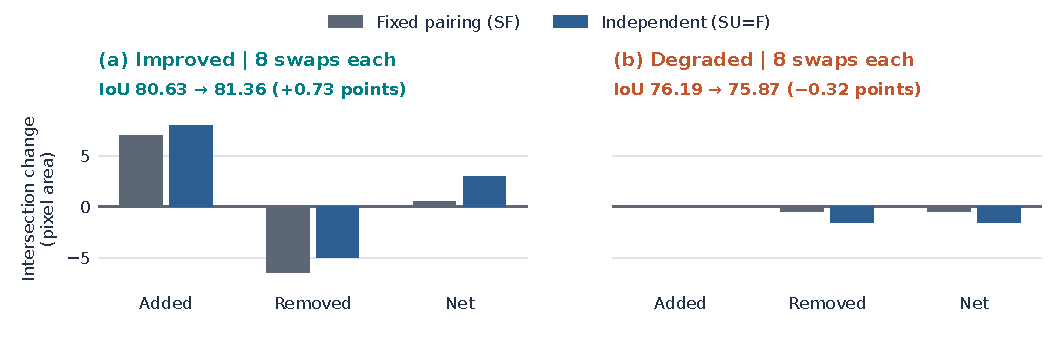
\includegraphics[width=0.82\textwidth]{figures/cvpr_20261126/dev705_overlap_cases.pdf}
\caption{Two observed RF-DETR DEV705 matches at the same edit count in seed 5217. Each arm adds eight pixels and removes eight. Bars report the intersection contributed by added native cells, the intersection lost in removed cells, and their net effect relative to the raw mask. IoU compares each complete edited mask with the same reference polygon. Cases are observed matches nearest the median within the positive and negative IoU differences, respectively, with the first image excluded when choosing the second case.}
\label{fig:dev-cases}
\par\vspace{7pt}
\includegraphics[width=0.79\textwidth]{\CaseAsset{gf3_matched_cases_binned.pdf}{gf3_cases_exact.pdf}}
\caption{Observed Gaofen-3 outcomes at matched dynamic-attraction counts, detector 5203 and occupancy head 5217. Two positive and two negative cases are selected by proximity to the continuous-IoU median within each sign among 425 eligible original matches, before inspection of the imagery. All illustrated edits add eight and remove eight native pixels. \CaseCaption{The public visual pools exact masks, reference coverage and signed changes to an \(8\times8\) spatial grid. The dashed binned reference can fragment a narrow footprint.}{The rows show native SAR crops with the author reference, native mask, attraction and learned predictions, and their signed differences.} Reported IoU and signed overlap are evaluated on the original grid using the author polygon.}
\label{fig:gf3-qual}
\end{figure*}

\begin{figure*}[!t]
\centering
\includegraphics[width=\textwidth]{\CaseAsset{pseg_budget_cases_binned.pdf}{pseg_budget_cases_exact.pdf}}
\caption{Fixed-count versus threshold writing on PSeg-SSDD. The labels Gain and Loss denote fixed count minus threshold. Native, threshold and fixed-count IoUs are 66.88, 56.40 and 62.26 in (A), and 56.04, 58.75 and 56.64 in (B). Cases were chosen near each sign's median continuous-IoU change. \CaseCaption{Columns show pooled reference occupancy, the threshold and fixed-count footprints, and the error map (threshold minus fixed count). Teal indicates lower error at the fixed count.}{The three columns use the same native SAR crop with the author polygon and the native, threshold, or fixed-count mask.} False-positive and false-negative percentages and IoU use the original polygon and cell grid.}
\label{fig:pseg-budget-cases}
\end{figure*}

\begin{figure*}[!t]
\centering
\includegraphics[width=0.86\textwidth]{\CaseAsset{rsdd74_segrefiner_cases_binned.pdf}{rsdd74_segrefiner_cases_SAR_PRIVATE.pdf}}
\caption{Observed gain and loss from the original SegRefiner-LR writer on Instance-RSDD, with the native and local occupancy masks for comparison. We select a different image nearest each sign's median difference over 39 eligible original matches. \CaseCaption{The public panels pool the original footprints and their changes onto an \(8\times8\) grid.}{The original author outline and the three mask predictions are overlaid on the same native SAR crop.} Continuous IoU and signed intersection changes are measured on the original grid.}
\label{fig:segrefiner-cases}
\end{figure*}


For seed 5217, freeing the pair assignment improves 1,012 of 1,461 fixed matches (69.3\%) and degrades 252 (17.2\%). The remaining 197 (13.5\%) differ by at most \(10^{-12}\) in continuous IoU. Fig.~\ref{fig:dev-cases} decomposes two median-sign cases using exact overlap. In (a), the independent additions recover one extra reference pixel-equivalent and the removals spare another 1.5. IoU gains 0.732 points. In (b), neither policy's additions recover any reference area. Independent selection removes one more pixel-equivalent of the hull and loses 0.316 IoU points. The second case illustrates a failure of occupancy ranking even though the independent writer maximizes estimated gain.

\subsection{Ranking differences on real Gaofen-3 vessels}


For the second detector's 425 eligible Gaofen-3 matches, seed 5217 improves 268 masks (63.1\%) over dynamic attraction, worsens 154 (36.2\%), and ties three. Fig.~\ref{fig:gf3-qual} shows where area is redistributed in four cases, all at eight swaps. In the first two, learned ranking increases net reference intersection by 2.93 and 3.71 native pixel areas over dynamic attraction. Continuous IoU rises from 78.13 to 78.83 and from 71.86 to 72.56. In the other two, equal-sized edits lose 1.30 and 3.00 pixel areas of intersection. IoU falls from 87.09 to 86.52 and from 68.14 to 67.58. The native masks provide a third reference in each row. The gains and losses measure covered polygon area on the image grid.

\subsection{Effects of whole-grid edit counts on PSeg-SSDD}


The whole-support count improves 209 of the 293 original eligible PSeg matches, worsens 76, and ties eight. In Fig.~\ref{fig:pseg-budget-cases}(A), the threshold output shrinks inward along the sides of the hull. Reducing 38 flips to 16 retains an additional \(17.87\) native pixel areas inside the reference, raising IoU from 56.40 to 62.26. The native mask has IoU 66.88. In (B), thresholding restores part of the narrow upper end and increases IoU from 56.04 to 58.75. Sixteen fixed-count changes reduce the false-positive fraction from 1.26\% to 0.22\% and lose \(7.96\) pixel areas of reference intersection, giving IoU 56.64.

\subsection{Whole-crop SegRefiner updates}


Among the 39 original geometry matches that entered SegRefiner-LR, 14 gain continuous IoU and 25 lose it. Fig.~\ref{fig:segrefiner-cases} shows the cases nearest the gain and loss medians. In (a), SegRefiner reduces the predicted extension beyond the lower end of the reference and increases IoU from 58.68 to 60.96. In (b), overlap is lost at both ends and along the narrow side, reducing IoU from 71.93 to 67.43. The local occupancy masks score 58.89 and 71.95 on the same references.

\subsection{Matched boundary edits on SAR-SSP}

\ifnativecases
\begin{figure*}[!t]
\centering
\includegraphics[width=0.94\textwidth]{local_figures/sarssp_private_cases.pdf}
\caption{Same-budget comparisons on observed SAR-SSP hulls. The rows use native SAR context and the author reference together with the actual fixed and independent writes. The pooled statistics and full matched denominator appear in Fig.~\ref{fig:sar-ssp-cases}.}
\label{fig:sar-ssp-native-cases}
\end{figure*}
\fi


Equal-count independent and distance-paired writing produce different masks for 52 of the 92 original matched hulls. Of the changed masks, independent writing improves discrete IoU in 21, reduces it in 15, and preserves it in 16. Fig.~\ref{fig:sar-ssp-cases} shows the distribution and spatial pattern of these changes. The signs of individual effects coexist with the small net AP change in Table~\ref{tab:sar-ssp}.

\begin{figure*}[t]
\centering
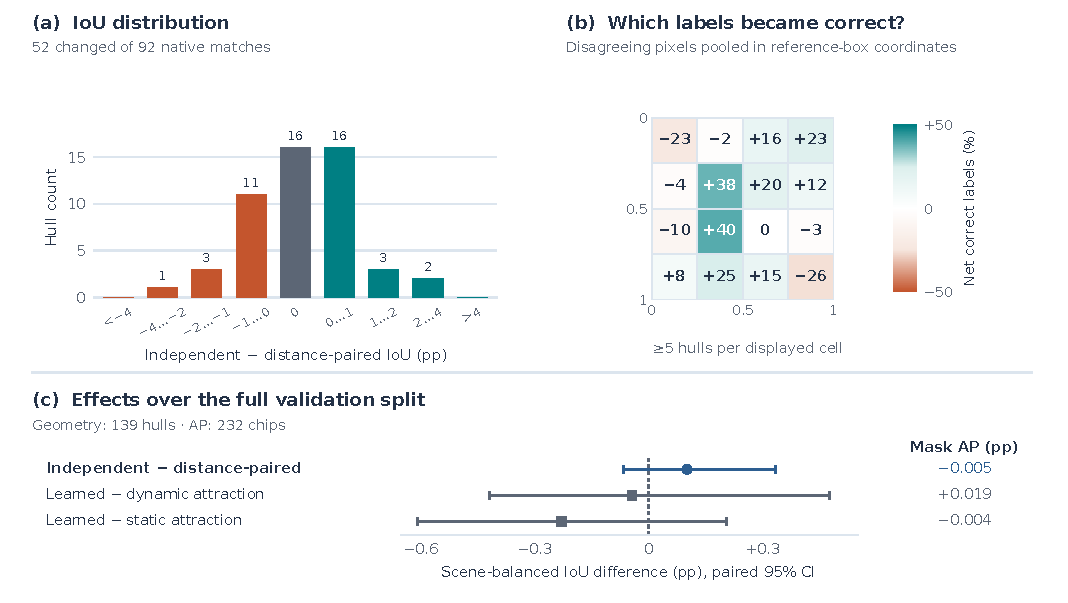
\includegraphics[width=0.95\textwidth]{figures/cvpr_20261126/sarssp_public_summary.pdf}
\caption{Observed SAR-SSP boundary edits. (a) Discrete IoU changes among the 52 original matches with different masks under the two equal-count policies. (b) Mean difference in the fraction of correct labels at disagreeing cells, evaluated within a normalized \(4\times4\) grid in each hull's image-axis-aligned enclosing rectangle. Each displayed cell pools at least five hulls. (c) Scene-balanced geometry differences over all 139 reference hulls with paired 95\% intervals and mask AP differences over all 232 chips.}
\label{fig:sar-ssp-cases}
\end{figure*}

\section{Ablation Studies}
\label{sec:ablation}
We vary the point scores, the add/remove choices and the pretrained writer in experiments that control different variables. The writer comparisons reuse frozen responses. Each ablation holds its candidate stream and its indicated budget fixed.

\subsection{Occupancy cues, label representation and head capacity}
On 412 detector-visible FIT109 matches, truth-ranked geometry reaches IoU 0.90 for 11 with fixed pairing, 27 with independent equal counts, and 38 with free add and delete counts. These are bounds on the original support. Limited gains from partner features and direct difference supervision at matched counts motivated the simpler occupancy head.

Our Atkinson adaptation~\cite{atkinson} uses a five-pixel radius and decay length. At 43,624 dynamic swaps on 6,159 FIT109 candidates, learned, dynamic and static ranks scored 53.344, 48.152 and 48.669 AP. Learned gains over dynamic were 1.104 IoU (\([0.788,1.446]\)) and \(-0.164\) AP90. Keeping each neighbor's gray-rank affinity gained 1.519 AP and 0.165 normalized intersection (\([0.080,0.264]\)) over averaging equal-distance affinities. Gray rank alone and learned occupancy gained 0.370 and 3.039 AP over aligned affinity. FIT109 trained the detector. Heads used five source-held-out folds.

On detector-held-out DEV705, the frozen all-FIT109 head and both attraction rules exchanged 262,802 pairs on 37,811 candidates, editing all 1,447 eligible matches. Learned, dynamic and static rankings scored 50.727, 48.299 and 48.396 AP. Learned ranking gained 5.353 AP75 and 1.150 IoU over dynamic (paired 27-prefix 95\% interval \([0.927,1.397]\)). Excluding four empty reference rasters gave a 2.434 AP gain.

On D-FINE FIT109, fractional labels gain 0.184 AP and 0.111 IoU over COCO rasters and 0.051 AP and 0.034 IoU over thresholding at 0.50, with one negative AP seed. On 74 Instance-RSDD images across three RF-DETR head seeds, full fractions scored 0.030 AP and 0.009 IoU below hardening all labels except 0.50 at equal counts (IoU interval \([-0.018,-0.002]\)), and gained 0.122 AP and 0.109 IoU over COCO rasters.

We retrained the point heads on FIT109 features from a frozen RF-DETR~\cite{rfdetr} detector trained with center-aligned target masks. Experiments use the official implementation, version 1.12.0. Three point-head initialization and sampling seeds share the same RF-DETR checkpoint, DEV705 population and 67,386 native mapped candidates. The 1,321- and 139,265-parameter heads use the same point features and each receives 200 updates in each refit. Table~\ref{tab:rfdetr} reports the COCO evaluation against 1,782 annotations and continuous IoU over 1,461 fixed matches, with equal weight for each of the 27 source-prefix groups. For the paired bootstrap we average the three seeds within each group before resampling groups.

\begin{table}[t]
\centering
\caption{RF-DETR DEV705. Entries are means over three point-head seeds, scaled by 100. Matched point policies use the same per-candidate edit count as the indicated reference.}
\label{tab:rfdetr}
\footnotesize
\begin{tabular}{@{}lrrr@{}}
\toprule
Mask policy & AP & AP75 & Fixed IoU\\
\midrule
N: Raw RF-DETR & 56.072 & 65.433 & 78.940\\
SF: Small head, fixed pairing & 56.006 & 65.264 & 78.889\\
SU=F: Independent, SF count & 56.912 & 66.844 & 79.528\\
SU: Independent, natural count & 56.865 & 66.785 & 79.537\\
LF=S: Large, fixed, SU count & 55.693 & 64.369 & 78.741\\
LU=S: Large, independent, SU count & 56.860 & 66.925 & 79.530\\
LW=S: Large, free-write, SU count & 56.669 & 66.893 & 79.390\\
NP=S: Native ranks, SU count & 55.935 & 64.767 & 78.786\\
\bottomrule
\end{tabular}
\end{table}

The three SU gains over the native detector are 0.808, 0.847, and 0.726 AP points. SU gains 0.598 continuous IoU points, with a paired source-group 95\% interval of \([0.513,0.698]\). With the small head and pair count held fixed, SU=F gains 0.906 AP and 0.639 IoU points over SF. The latter has interval \([0.548,0.743]\). The natural-count small-head SU policy gains 0.197 AP and 0.147 IoU points over the same-count large-head writer LW=S. The IoU interval is \([-0.041,0.415]\). These fall below the prespecified comparison margins of 0.30 AP and 0.20 IoU points, so the primary policy does not advance under the original rule. Holding the large head and count fixed, LU=S gains 0.192 AP and 0.139 continuous IoU points over LW=S.

Among the 86 native matches above 0.90, 9, 9, and 10 fall to or below the threshold across the three heads. A further 29, 21, and 18 matches cross upward from at or below 0.90. The observed effects apply to the shared frozen carrier and point training budget. The stronger detector experiment supports the effect of freeing the fixed pair assignment, while the value of preserving the edit area relative to a competitive point writer remains unresolved.





At each head seed's realized natural-policy counts, ranking by true pixel occupancy would improve continuous IoU by 2.111 points over SU, with a paired interval of \([1.863,2.383]\). Varying the number of additions and removals at the same total count yields an additional 1.001 points, with interval \([0.814,1.224]\). These bounds retain the 1,461 original matched objects and the same endpoint support. With learned ranks frozen, a quota-only oracle gains 1.264 points over SU. All bounds are conditional on native matches.

Query features gain 0.352 AP and 0.073 IoU at fixed FIT109 counts. The IoU interval crosses zero. Zero padding and within-candidate permutation each give higher AP.

Five group-held-out FIT109 PointRend heads (200 updates each) gain 2.440 full-paste AP over coarse paste, 3.851 below native. At equal counts, balanced independent editing gains 1.047 AP and 0.262 IoU over fixed pairs (\([0.131,0.406]\)), and 0.938 AP and 0.084 IoU over unconstrained-area editing (\([-0.039,0.202]\)). The detector trained on FIT.

On HRSID FIT36, five registered shift views share the original queries, native support, 166 fixed matches and 1,209 swaps. The second-worst signed rank loses 0.333 continuous IoU points to the mean-logit rank (\([-0.489,-0.149]\)).

\subsection{Independent addition and removal locations}
\label{sec:side-ablation}

To isolate each side of the decision, we construct four masks from the same endpoints and head scores. The first takes both sides from fixed pairing. The middle two use independent ranks on just one side and retain the other side's fixed selection. The fourth uses independent ranks on both sides. Every cell count, confidence and native foreground area is matched. This intervention changes two parts of the action rule from Eq.~\eqref{eq:independent-estimated-gain}. The addition and removal contributions to \(g\) in Eq.~\eqref{eq:intersect-changes} add exactly on a fixed hull. Mask AP can have an interaction because matching occurs across a ranked detection list.

\begin{table*}[t]
\centering
\caption{Add-side and remove-side ablation on Instance-RSDD at fixed counts. Entries are mask AP points. The 42-chip date-separated view is nested in the 74-chip reserve. Bold values denote the largest measured AP in each row.}
\label{tab:signed-side-ablation}
\footnotesize
\setlength{\tabcolsep}{5pt}
\begin{tabular}{@{}llrrrr@{}}
\toprule
View & Point-head seed & Both fixed & Independent add only & Independent remove only & Both independent\\
\midrule
Gaofen-3, 583 chips & 5217 & 61.036 & 61.331 & 61.286 & \textbf{61.518}\\
Gaofen-3, 583 chips & 5218 & 60.984 & 61.207 & 61.302 & \textbf{61.468}\\
Reserve, 74 chips & 5217 & 58.278 & 58.545 & 58.426 & \textbf{58.714}\\
Date-separated, 42 chips & 5217 & 61.283 & 61.769 & 61.698 & \textbf{62.123}\\
\bottomrule
\end{tabular}
\end{table*}

\begin{figure}[t]
\centering
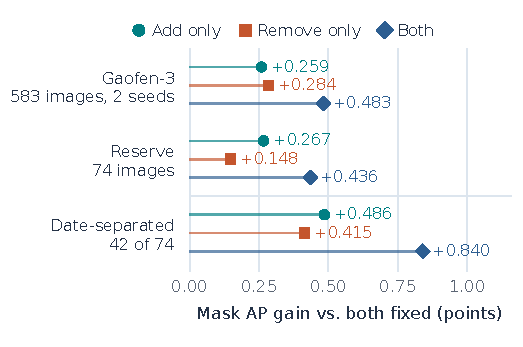
\includegraphics[width=\columnwidth]{figures/cvpr_20261126/independent_sides_ablation.pdf}
\caption{AP changes from switching one or both sides to independent selection. The reference within each row is the fixed-pair policy. The Gaofen-3 values average the two frozen point-head seeds. All policies have the same add count, remove count and final area.}
\label{fig:signed-side-ablation}
\end{figure}

Table~\ref{tab:signed-side-ablation} and Fig.~\ref{fig:signed-side-ablation} show improvement from each single-side rule and the highest measured AP when both sides are independent. The joint rule also improved fixed-match continuous IoU over each single-side candidate in the main Gaofen-3 and reserve views. The AP interaction is small and changes sign between cohorts. These results support distinct effects of editing each side. Their relative sizes depend on the cohort and metric.

At fixed head and count, freeing both sides versus additions alone gained 0.224 AP and 0.175 IoU on Gaofen-3 (two-seed means, \([0.130,0.222]\)) and 0.169 AP and 0.170 IoU on the 74 chips (\([0.108,0.251]\)). Over deletions alone, gains were 0.199 AP and 0.085 IoU (\([0.049,0.120]\)) and 0.288 AP and 0.148 IoU (\([0.042,0.252]\)). AP rose at every seed. Both date-separated IoU intervals stayed positive.

Under the same dynamic budget, learned additions and removals each improve intersection on DEV705 (\(+0.308\) and \(+0.446\) points of hull area) and each lower it on PSeg-SSDD and UEIKAP342. External comparisons between the two sides have intervals spanning zero. A \href{https://github.com/bingzhi495-creator/SAR-SEAL-research/blob/3f8f738/research_round_20260925_global/ATTRACTION_LOCAL_CORRECTION_ACTUAL_20261123.md}{ridge adjudicator} fit on 4,063 disputed FIT109 pairs gains 0.018 IoU over scores alone on DEV705 (\([0.008,0.028]\)); on deduplicated PSeg, its interval spans zero and static attraction leads by 0.115 AP.

With frozen Phoenix scores, independent selection improves over fixed pairing by 0.486 AP and 0.327 continuous IoU on Instance-RSDD, and 0.731 AP and 0.595 IoU on PSeg-SSDD. We then allow posterior-optimal re-pairing under the original per-candidate maximum swap distance. This gains 0.250 and 0.534 AP. Removing that cap adds 0.236 and 0.197 AP, below the prespecified 0.30 points in both full cohorts. Residual IoU gains are 0.197 (\([0.063,0.324]\)) and 0.280 (\([0.171,0.398]\)). PSeg static attraction still leads the independent arm by 0.195 AP at that count.

\subsection{Pretrained writer support, count and signed allocation}
\begin{table*}[t]
\centering
\caption{Support and count ablation for a single frozen Phoenix response. Reported AP and fixed continuous IoU are points. The four factorial rows use the same positive-budget slots; other detections retain the native mask. The balanced row retains the narrow support and total count.}
\label{tab:phoenix-factors}
\footnotesize
\setlength{\tabcolsep}{5pt}
\begin{tabular}{@{}llrrr@{\quad}rrr@{}}
\toprule
 & & \multicolumn{3}{c}{Instance-RSDD reserve (74)} & \multicolumn{3}{c}{PSeg-SSDD official (232)}\\
\cmidrule(lr){3-5}\cmidrule(l){6-8}
Support & Writing rule & Flips & AP & IoU & Flips & AP & IoU\\
\midrule
Whole grid & Author threshold & 2,042,908 & 49.085 & 69.428 & 3,391,327 & 13.922 & 65.739\\
Whole grid & Count, free split & 59,800 & 58.478 & 78.890 & 147,540 & 16.447 & 69.741\\
Narrow & Author threshold & 114,328 & 58.498 & 79.260 & 270,637 & 15.866 & 68.996\\
Narrow & Count, free split & 59,800 & 58.787 & 79.171 & 147,540 & 16.380 & 69.417\\
Narrow & Count, equal signs & 59,800 & 58.976 & 79.253 & 147,540 & 18.222 & 70.568\\
\bottomrule
\end{tabular}
\end{table*}

To test area conservation under a common edit limit, we keep the same Phoenix probabilities, endpoints and \(2k\) flips for every candidate. We rank addition gains by \(p-0.50\) and removal gains by \(0.50-p\), where \(p\) is the frozen Phoenix occupancy. Sorted prefixes determine the maximum estimated pixel-correctness gain under each quota. With no constraint on \(d\), the 59,800 flips add a net 23,828 foreground cells across all predictions. Relative to that policy, strict balance gains 0.190 AP and 0.083 continuous IoU (\([-0.191,0.401]\)). The written masks differ for 45 fixed hulls in 11 sensor--date blocks. A two-cell tolerance on \(|d|\) gives 58.856 AP, compared with 58.976 for strict balance and 58.787 for free allocation. All three retain the 81 original matches. On HRSID DEV705, free allocation with a source-trained occupancy head gains 0.212 AP and 0.009 continuous IoU over balance at 631,020 fixed flips in a single fit. The estimated effect is small on the Instance-RSDD reserve and changes direction in the HRSID comparison, which also uses a different ranking field. The much larger loss under whole writing calls for separate tests of support and flip count.

We cross the writable support with the flip rule using the same fifth-iteration Phoenix posterior for each of the 4,107 positive-budget candidates. All other candidates retain the native mask. Narrow support uses the original sampled endpoints. Whole support covers the original image grid. The threshold writer applies the author's binary decision at every available location. Exact-count writing uses the same \(2k\) flips as the original narrow run and maximizes summed pixel-correctness gain with free signed counts. The narrow exact-count masks and the whole threshold masks reproduce their respective archived masks on all 4,107 candidates. All 259,242 recorded probabilities also match.

\begin{figure*}[!t]
\centering
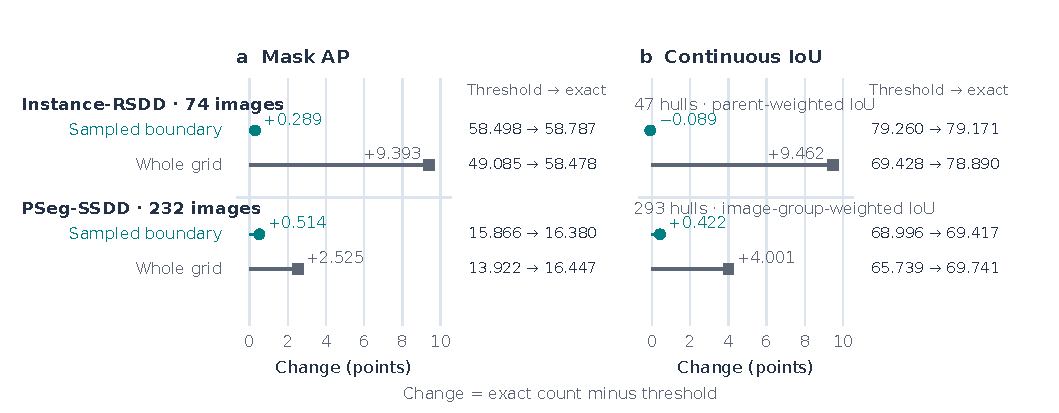
\includegraphics[width=\textwidth]{figures/cvpr_20261126/phoenix_budget_by_dataset.pdf}
\caption{Writable support and edit count on two frozen detector streams. Within each dataset, all four policies use the same editable candidates and Phoenix probabilities. Mask AP uses the full native candidate stream. Continuous IoU weights parent scenes equally over 47 original eligible matches on Instance-RSDD and decoded-image groups equally over 293 matches on PSeg-SSDD. Both panels use the same horizontal difference scale. The columns give the original threshold and exact-count scores.}
\label{fig:phoenix-support-budget}
\end{figure*}

On whole support, imposing the old count reduces flips from 2,042,908 to 59,800 and raises AP from 49.085 to 58.478 (Fig.~\ref{fig:phoenix-support-budget}). Continuous IoU increases by 9.462 points (paired 95\% interval \([6.329,13.283]\)). False positive area drops by 33.131 points of reference area (\([-49.245,-19.298]\)), and missed area changes by \(+2.957\) points (\([-0.058,5.863]\)). The number of hulls rematched at IoU 0.50 recovers from 77 to 81. The exact-count rule uses 44,158 cells outside the sampled support. Relative to native, its AP improves by 0.201 points while AR100 is 0.494 points lower.

On narrow support the count constraint changes AP by \(+0.289\) and IoU by \(-0.089\) points. The count effect is 9.105 AP points larger on whole support. The continuous-IoU interaction is 9.551 points (\([6.398,13.365]\)). The equal-count comparison of narrow and whole writing gives \(+0.309\) AP and \(+0.281\) IoU for the narrow writer, with interval \([-0.025,0.666]\). On the 42 date-separated chips, the whole-support count effect remains positive at 12.920 AP and 10.672 IoU points.

On PSeg-SSDD, we switch to frozen D-FINE and keep the original dynamic-attraction counts on the 11,054 editable candidates. The whole-grid threshold writer performs 3,391,327 flips. The exact-count writer performs 147,540, raising AP from 13.922 to 16.447 and fixed continuous IoU by 4.001 points (\([2.644,5.382]\)). Foreground outside the reference falls by 7.382 points of reference area (\([-11.989,-3.621]\)). At IoU 0.50, rematching covers 404 hulls instead of 407, and the number retaining their original candidate rises from 377 to 394. On 222 images after excluding historical exact overlaps, AP and continuous IoU rise by 2.694 and 4.095 points under the same count comparison. All comparisons retain the official allocation's full candidate stream for the applicable images.

The narrow exact-count writer on PSeg-SSDD improves on narrow thresholding by 0.514 AP and 0.422 IoU points (\([0.253,0.595]\)). At the fixed count it scores 0.067 AP lower than the whole writer and loses 0.323 IoU points (\([-0.560,-0.111]\)). The count effect on whole support exceeds the effect on narrow support by 2.011 AP and 3.580 IoU points (IoU interval \([2.316,4.887]\)). Applying the bound therefore reduces threshold-write errors in both datasets, with different residual errors. On PSeg-SSDD, whole-support exact-count Phoenix remains 1.528 AP below native D-FINE and 1.970 AP below matched static attraction.

At the same 147,540 flips on the sampled endpoints, assigning half to each side raises Phoenix AP from 16.380 to 18.222 on PSeg-SSDD. The paired continuous IoU gain is 1.151 points (\([0.701,1.594]\)). The writers differ on 283 of 293 fixed matches and in 137 of 143 decoded-image groups. Missed area falls by 1.428 points of reference area and false-positive area rises by 0.340 points. The balanced writer trails matched static attraction by 0.195 AP and 0.076 IoU points (\([-0.246,0.105]\)). Compared with the matched learned head, it gives 0.109 lower AP and 0.186 higher IoU (\([0.036,0.339]\)). After excluding ten historical exact overlaps, the balanced writer gains 2.093 AP and 1.232 IoU points over free allocation (\([0.762,1.682]\)). The matched differences relative to static and learned rankings retain their directions.

\section{Discussion and Reproducibility}
\subsection{Transfer and Reference Dependence}
The equal-count comparison identifies the effect of choosing different positions within the same boundary support. Its AP gains recur on the Gaofen-3 subset for two downstream fits sharing initialization and evaluation scenes. Effects are smaller on PSeg-SSDD and SAR-SSP. On the 232 historical SSDD images, switching from PSeg to SPSD reverses the AP effect of the area-preserving natural-count endpoint writer relative to the native masks. The fixed-candidate comparison attributes most of the corresponding IoU shift to edited cells with conflicting labels (Fig.~\ref{fig:reference-disagreement}). Boundary gains should therefore be read together with the overlap convention and reference population.

The HRSID official reevaluation and the SAR-SSP validation cohort had prior evaluation exposure. The two Gaofen-3 detector fits share target scenes. Table~\ref{tab:cohorts} and the reserve protocol identify where parent IDs and sensor--date keys separate the evaluated views. Native, local and Phoenix masks have been frozen for 12 prospectively selected Umbra windows. A separate 24-collect supplemental cohort has also completed native-intake verification and frozen edit replay. Both cohorts await independent reference scoring.

\subsection{Proposal Coverage and Edit Constraints}
Two limits appear on SAR-SSP. First, only one of the 47 unmatched hulls crosses mask IoU 0.50 under reference-guided edits within the original support and exchange cap. The 164 raw queries add box-level coverage for two of the 47 hulls. In a separate mask ceiling, arbitrary changes inside the existing boxes recover nine hulls at fixed area and a further 19 if area can vary. These per-hull ceilings allow candidate reuse. Second, on the 92 original matches, observed endpoint counts permit a reference-optimal gain of 1.187 scene-balanced discrete IoU points over learned independence and 0.895 points over reference-optimal distance pairing. At least some retained proposals have useful local headroom, while broader support or new proposals are necessary for many misses. On UEIKAP, only 17 of 139 released hulls have positive-budget native matches.

The stock SegRefiner experiments separate where a deletion occurs from how many deletions are made. Keeping the stock additions and replacing its deletion sites by reference-guided sites at the same count improves IoU by 5.594 and 3.512 points on the evaluated Instance-RSDD and PSeg-SSDD matches, respectively. Allowing fewer deletions adds 4.256 and 4.189 points. A label-free cap limits retained deletions to the smaller of the stock addition and deletion counts. Uniform selection under the cap gains 0.907 and 0.878 AP points over the stock writer. The capped writers remain below addition-only and the local occupancy writer on both evaluated cohorts. The location and count of deletion errors both matter in these fixed-response comparisons.

\subsection{Topology and Physical Interpretation}
An equal-area write can still split a component, introduce a hole or increase overlap with a neighboring vessel. Natural-count edits increased the number of holes in 1,544 of 10,466 edited PSeg masks, compared with 519 when the native response ranked the same number of edits. Conversely, 24 of the 26 Instance-RSDD hulls harmed by stock SegRefiner deletion retained their component and hole counts. Topology counters alone miss many local extent errors. At the small-size limit, all 107 nonempty candidate masks in the Schwegmann set~\cite{schwegmann} fell below the editor's 32-cell area floor.

The physical-sizing checks have limited common coverage. Of 142 NovaSAR AIS chips~\cite{nastar}, 34 yielded common mask spans and 17 supported positive-budget edits. Equal-count independence changed absolute length error by \(+0.204\)~m (\([-0.110,0.581]\)~m). The 25 common Sentinel-1A cases in the Gulf data~\cite{gulf} gave a nominal MAE change of \(-0.168\)~m (\([-1.523,1.692]\)~m). The 23-case heading sensitivity still retained a mean geolocated length excess of 71.27~m after using AIS headings. The IoU gains in the segmentation experiments therefore provide insufficient evidence for improved physical sizing.

\subsection{Computation and Repeatability}
The D-FINE CUDA detector and postprocessor took 11.74\,s over 232 PSeg images. With detector outputs already loaded, exact-equivalent interpolation reduced single-thread local refinement from 158.8 to 104.3\,ms/image. On the 74 Instance-RSDD chips, occupancy writing, equal-count PointRend and whole-RoI PointRend took 227.1, 1,221.5 and 1,049.2\,ms/image over two single-thread passes. The PointRend hybrid renders the whole RoI before constrained writing. In a separate six-pass timing from cached endpoints, occupancy scores, budgets and pairings, distance-first, bounded and independent selection plus RLE writing take 26.1, 138.6 and 27.4 ms/image on the same logical CPU, respectively.

Frozen Phoenix took 1,404.48\,s on the PSeg cohort with four two-thread CPU workers, five iterations and 11,054 prompts. Stock SegRefiner-LR took 454.18\,s over 74 Instance-RSDD images on an RTX 3090 Ti and 13,420.42\,s on the PSeg cohort under shared workstation load. These are observed wall times under the reported systems and workloads. The \href{https://github.com/bingzhi495-creator/SAR-SEAL-research}{repository} provides code, configurations, data access notes and score summaries. Independent replay reproduced 3,434 table entries for the HRSID official split and Instance-RSDD 740, plus 1,470 entries on the 74-chip reserve for detector 5202 and head 5217. Reproduction uses the original annotations and the designated frozen weights.

\section{Conclusion}
At matched signed counts, independent endpoint selection improves fixed hull overlap and mask AP over distance-first pairing on HRSID and in the evaluated Instance-RSDD subsets. On the historical 74-chip reserve, the AP and continuous overlap gains also hold against exact bounded re-pairing with frozen RF-DETR and D-FINE. At one pixel both pipelines improve Boundary IoU with bounded re-pairing over distance-first selection, while the additional change under independent selection remains uncertain. In the fixed-match boundary diagnostic, one-pixel gains are supported for GF-3 detector 5202 and the 74-chip reserve. The second GF-3 fit has an interval that spans zero at one pixel and a positive two-pixel interval. The gains on the common Gaofen-3 images recur for two downstream detector fits that share initialization. The same comparison produces small AP differences on PSeg-SSDD and SAR-SSP. On the 232 historical SSDD images, changing from the PSeg to the SPSD reference reverses the AP effect of the area-preserving natural-count endpoint writer relative to the native masks. The small number of editable matches on UEIKAP and the proposal-coverage analysis on SAR-SSP identify a separate limit on what local editing can recover.

At fixed total flips, a variable split improves mean AP and fixed-match raster IoU across three head fits under both labels of the same SSDD development images. On SAR-SSP, the frozen policy reduces missed area and increases false-positive area. Its paired IoU interval spans zero and the transfer criterion is unmet.

The pretrained-refiner comparisons isolate the effect of the edits themselves. Limiting whole-grid Phoenix writes reduces excess foreground changes on both evaluated datasets. For SegRefiner-LR, separately scoring additions and removals exposes deletion losses that a per-candidate cap partly recovers. These experiments show why endpoint ranking, signed allocation, and candidate coverage should be measured separately when evaluating local mask refinement.

\section*{Data and Code Availability}
The project repository provides executable analysis code, frozen-protocol definitions and aggregate results. The original releases provide evaluation imagery and contour annotations under their respective access terms. Reproduction of the fixed-mask comparisons uses the specified detector weights, original image splits, released contours and the versioned capture and replay procedures.

\section*{Acknowledgment}
OpenAI Codex assisted with English drafting and revision in the abstract, Sections I--IX, and the figure captions. It also assisted in generating the vector-figure scripts, schematic layouts and experimental analysis code. The conceptual diagrams use illustrative cells and worked examples. The data figures use observed results and identify the spatial pooling applied in the displayed views.

\IEEEtriggeratref{21}
\begin{thebibliography}{34}
\bibitem{hrsid} S. Wei, X. Zeng, Q. Qu, M. Wang, H. Su, and J. Shi, ``HRSID: A high-resolution SAR images dataset for ship detection and instance segmentation,'' \emph{IEEE Access}, vol. 8, pp. 120234--120254, \href{https://doi.org/10.1109/ACCESS.2020.3005861}{2020}.
\bibitem{rsdd} X. Yang, Q. Zhang, Q. Dong, Z. Han, X. Luo, and D. Wei, ``Ship instance segmentation based on rotated bounding boxes for SAR images,'' \emph{Remote Sens.}, vol. 15, no. 5, Art. no. 1324, \href{https://doi.org/10.3390/rs15051324}{2023}.
\bibitem{gao2024} F. Gao, X. Han, J. Wang, J. Sun, A. Hussain, and H. Zhou, ``SAR ship instance segmentation with dynamic key points information enhancement,'' \emph{IEEE J. Sel. Topics Appl. Earth Observ. Remote Sens.}, vol. 17, pp. 11365--11385, 2024. \href{https://doi.org/10.1109/JSTARS.2024.3383779}{10.1109/JSTARS.2024.3383779}.
\bibitem{dfine} A. Saakyan and D. Solntsev, ``D-FINE-seg: Object detection and instance segmentation framework with multi-backend deployment,'' \href{https://arxiv.org/abs/2602.23043}{arXiv:2602.23043}, 2026.
\bibitem{rfdetr} I. Robinson, P. Robicheaux, M. Popov, D. Ramanan, and N. Peri, ``RF-DETR: Neural architecture search for real-time detection transformers,'' in \emph{Proc. Int. Conf. Learn. Represent. (ICLR)}, 2026.
\bibitem{ssdd} T. Zhang \emph{et al.}, ``SAR Ship Detection Dataset (SSDD): Official release and comprehensive data analysis,'' \emph{Remote Sens.}, vol. 13, no. 18, Art. no. 3690, 2021. \href{https://doi.org/10.3390/rs13183690}{10.3390/rs13183690}.
\bibitem{drsnet} Q. Zhang and Z. Han, ``DRSNet: Rotated-ROI ship segmentation for SAR images based on dual-scale cross attention,'' \emph{IEEE Geosci. Remote Sens. Lett.}, vol. 21, pp. 1--5, 2024. \href{https://doi.org/10.1109/LGRS.2024.3420251}{10.1109/LGRS.2024.3420251}.
\bibitem{gldet} H. Chang, X. Fu, P. Lang, K. Guo, J. Dong, and S. Chang, ``GLDet: Real-time SAR ship detector based on global semantic information enhancement and local gradient information mining,'' \emph{IEEE Trans. Geosci. Remote Sens.}, vol. 63, Art. no. 5209020, 2025. \href{https://doi.org/10.1109/TGRS.2025.3559551}{10.1109/TGRS.2025.3559551}.
\bibitem{aranet} S. Chang, P. Lang, H. Chang, C. Zhao, J. Yang, J. Dong, and X. Fu, ``ARANet: A unified representation alignment framework for SAR ship instance segmentation,'' \emph{IEEE J. Sel. Topics Appl. Earth Observ. Remote Sens.}, vol. 19, pp. 28679--28694, 2026. \href{https://doi.org/10.1109/JSTARS.2026.3720719}{10.1109/JSTARS.2026.3720719}.
\bibitem{gcie} W. Luo, J. Lan, Y. Zeng, and W. Xiong, ``GCIE-Net: A global and channel information-enhanced network for ship instance segmentation in SAR images,'' \emph{Remote Sens.}, vol. 18, no. 15, Art. no. 2512, 2026. \href{https://doi.org/10.3390/rs18152512}{10.3390/rs18152512}.
\bibitem{dacf} S. Yang, X. Zhang, W. An, Z. Li, and N. Chen, ``DACF-Net: A dynamic attention and context fusion network with geometry-aware multi-scale refinement for SAR ship instance segmentation,'' \emph{Int. J. Digit. Earth}, vol. 19, no. 2, Art. no. 2696657, 2026. \href{https://doi.org/10.1080/17538947.2026.2696657}{10.1080/17538947.2026.2696657}.
\bibitem{dsr} S.-W. He, W. Xiong, and L.-B. Yao, ``SAR ship instance segmentation method in complex scenes jointly driven by differential physical fields and structured graph reasoning,'' \emph{Acta Electronica Sinica}, pp. 1--11, 2026. \href{https://doi.org/10.12263/DZXB.20260699}{10.12263/DZXB.20260699}.
\bibitem{atkinson} P. M. Atkinson, ``Sub-pixel target mapping from soft-classified, remotely sensed imagery,'' \emph{Photogramm. Eng. Remote Sens.}, vol. 71, no. 7, pp. 839--846, 2005. \href{https://doi.org/10.14358/PERS.71.7.839}{10.14358/PERS.71.7.839}.
\bibitem{xu} Y. Xu and B. Huang, ``A spatio-temporal pixel-swapping algorithm for subpixel land cover mapping,'' \emph{IEEE Geosci. Remote Sens. Lett.}, vol. 11, no. 2, pp. 474--478, 2014. \href{https://doi.org/10.1109/LGRS.2013.2268153}{10.1109/LGRS.2013.2268153}.
\bibitem{rankseg} B. Dai and C. Li, ``RankSEG: A consistent ranking-based framework for segmentation,'' \emph{J. Mach. Learn. Res.}, vol. 24, no. 224, pp. 1--50, \href{https://www.jmlr.org/papers/v24/22-0712.html}{2023}.
\bibitem{pointrend} A. Kirillov, Y. Wu, K. He, and R. Girshick, ``PointRend: Image segmentation as rendering,'' in \emph{Proc. IEEE/CVF Conf. Comput. Vis. Pattern Recognit. (CVPR)}, 2020, pp. 9799--9808.
\bibitem{segfix} Y. Yuan, J. Xie, X. Chen, and J. Wang, ``SegFix: Model-agnostic boundary refinement for segmentation,'' in \emph{Proc. Eur. Conf. Comput. Vis. (ECCV)}, 2020, pp. 489--506.
\bibitem{bpr} C. Tang, H. Chen, X. Li, J. Li, Z. Zhang, and X. Hu, ``Look closer to segment better: Boundary patch refinement for instance segmentation,'' in \emph{Proc. IEEE/CVF Conf. Comput. Vis. Pattern Recognit. (CVPR)}, 2021, pp. 13926--13935.
\bibitem{refinemask} G. Zhang, X. Lu, J. Tan, J. Li, Z. Zhang, Q. Li, and X. Hu, ``RefineMask: Towards high-quality instance segmentation with fine-grained features,'' in \emph{Proc. IEEE/CVF Conf. Comput. Vis. Pattern Recognit. (CVPR)}, 2021, pp. 6861--6869.
\bibitem{sharpcontour} C. Zhu, X. Zhang, Y. Li, L. Qiu, K. Han, and X. Han, ``SharpContour: A contour-based boundary refinement approach for efficient and accurate instance segmentation,'' in \emph{Proc. IEEE/CVF Conf. Comput. Vis. Pattern Recognit. (CVPR)}, 2022, pp. 4392--4401.
\bibitem{quber} S. Back, S. Lee, K. Kim, J. Lee, S. Shin, J. Maeng, and K. Lee, ``High-quality unknown object instance segmentation via quadruple boundary error refinement,'' in \emph{Proc. IEEE Int. Conf. Robot. Autom. (ICRA)}, 2025, pp. 13574--13581, doi: 10.1109/ICRA55743.2025.11127393.
\bibitem{phoenix} B. Kim and S. J. Hwang, ``Learning from adversity: Semantic-aware mask refinement through adversarial perturbation,'' in \emph{Proc. Eur. Conf. Comput. Vis. (ECCV)}, 2026, pp. 75--92. \href{https://doi.org/10.1007/978-3-032-37520-9_5}{10.1007/978-3-032-37520-9\_5}.
\bibitem{segrefiner} M. Wang, H. Ding, J. H. Liew, J. Liu, Y. Zhao, and Y. Wei, ``SegRefiner: Towards model-agnostic segmentation refinement with discrete diffusion process,'' in \emph{Adv. Neural Inf. Process. Syst.}, vol. 36, 2023. \href{https://proceedings.neurips.cc/paper_files/paper/2023/hash/fc0cc55dca3d791c4a0bb2d8ddeefe4f-Abstract-Conference.html}{Proceedings}.

\bibitem{rsddsar} C. Xu \emph{et al.}, ``RSDD-SAR: Rotated ship detection dataset in SAR images,'' \emph{J. Radars}, vol. 11, no. 4, pp. 581--599, 2022. \href{https://doi.org/10.12000/JR22007}{10.12000/JR22007}.
\bibitem{ueikap} A. Mazzeo \emph{et al.}, ``UEIKAP dataset,'' Zenodo, ver. 1.0, \href{https://doi.org/10.5281/zenodo.18391027}{2026}.
\bibitem{schwegmann} C. P. Schwegmann, W. Kleynhans, B. P. Salmon, L. W. Mdakane, and R. G. V. Meyer, ``Very deep learning for ship discrimination in Synthetic Aperture Radar imagery,'' in \emph{Proc. IEEE Int. Geosci. Remote Sens. Symp. (IGARSS)}, 2016, pp. 104--107. \href{https://doi.org/10.1109/IGARSS.2016.7729017}{10.1109/IGARSS.2016.7729017}.
\bibitem{nastar} B. Hosseiny, K. Kamirul, O. Pappas, and A. Achim, ``NASTaR: A NovaSAR-based automated ship target recognition dataset,'' \emph{IEEE Geosci. Remote Sens. Lett.}, vol. 23, Art. no. 1502605, 2026. \href{https://doi.org/10.1109/LGRS.2026.3679941}{10.1109/LGRS.2026.3679941}.
\ifnativecases\else\newpage\fi
\bibitem{gulf} M. Shaya, ``SAR Ship Gulf: Sentinel-1 GRD ship chips with AIS labels,'' Zenodo, ver. 1, 2026. \href{https://doi.org/10.5281/zenodo.21000650}{10.5281/zenodo.21000650}.

\bibitem{slgsea} R. Deng, T. Zhang, G. Gao, L. Zhang, S. Wei, and X. Zhang, ``SLGSea: Spatialized language guidance with scattering-aware query construction for ship--sea--land panoptic segmentation in SAR imagery,'' project repository and dataset release. \href{https://github.com/deng1218/SLGSea}{Code and data}.
\bibitem{mansour2026} I. Mansour, F. Sica, and M. Schmitt, ``Prompting foundation models for zero-shot ship instance segmentation in SAR imagery,'' \emph{arXiv:2604.17920}, \href{https://arxiv.org/abs/2604.17920}{2026}.
\bibitem{airsarship} X. Sun, Z. Wang, Y. Sun, W. Diao, Y. Zhang, and K. Fu, ``AIR-SARShip-1.0: High-resolution SAR ship detection dataset,'' \emph{J. Radars}, vol. 8, no. 6, pp. 852--862, 2019. \href{https://doi.org/10.12000/JR19097}{10.12000/JR19097}.
\bibitem{rankrma} Z. Wang and B. Dai, RankSEG-RMA: An efficient segmentation algorithm via reciprocal moment approximation, in \emph{Adv. Neural Inf. Process. Syst.}, vol. 38, 2025. \href{https://doi.org/10.52202/085713-5452}{10.52202/085713-5452}.
\bibitem{rankdep} Z. Wang and B. Dai, ``On the relaxation of conditional independence assumption for image segmentation,'' \href{https://arxiv.org/abs/2609.38930}{arXiv:2609.38930}, 2026.
\bibitem{boundaryiou} B. Cheng, R. Girshick, P. Doll{\'a}r, A. C. Berg, and A. Kirillov, ``Boundary IoU: Improving object-centric image segmentation evaluation,'' in \emph{Proc. IEEE/CVF Conf. Comput. Vis. Pattern Recognit. (CVPR)}, 2021. \href{https://arxiv.org/abs/2103.16562}{arXiv:2103.16562}.
\end{thebibliography}
\end{document}
